% !TeX root = ../../tesi.tex

%Background Material
\chapter{Background Material}

\section{Computer Vision}
% !TeX root = ../../tesi.tex

Computer vision is a subfield of artificial intelligence (AI) that equips machines with the ability to process, analyze and interpret visual inputs such as images and videos. It uses machine learning to help computers and other systems derive meaningful information from visual data.\cite{ibm_what_nodate}

Object detection and image segmentation are two fundamental tasks in the field of computer vision, widely used for scene understanding and automated visual analysis. While both aim at identifying relevant objects within an image, they differ significantly in terms of output representation, computational complexity, and application scope.

\subsection{Object detection}
Object detection \cite{ibm_what_nodate} aims to pinpoint where objects are in digital images. It melds two learning techniques:
\begin{itemize}
    \item \textbf{Object localization} identifies the location of specific objects in an image by drawing bounding boxes around them.
    \item \textbf{Image classification} distinguishes the category to which objects belong.
\end{itemize} 
\begin{figure}[h]
    \centering
    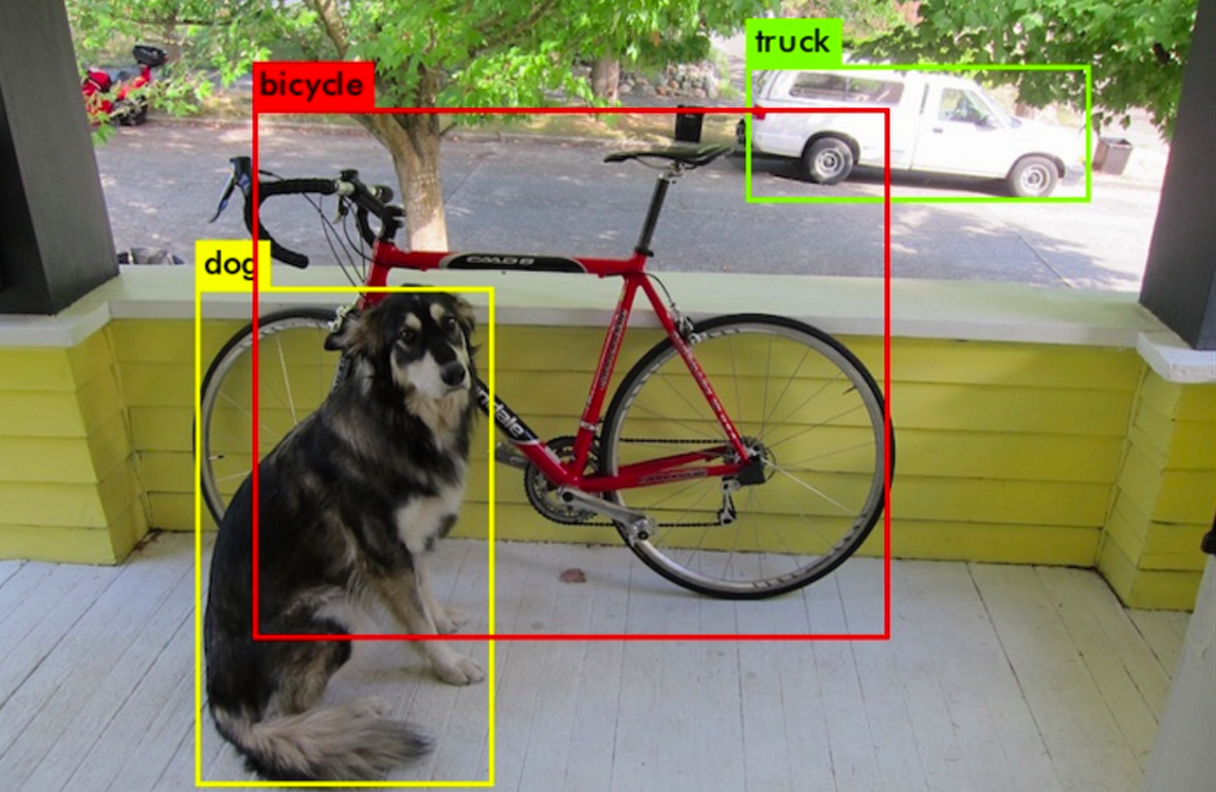
\includegraphics[scale=0.25]{images/object-detection.png}
    \caption{In the image, the detected objects are enclosed by bounding boxes \\and annotated with their corresponding class labels}
    \label{fig:object-detection}
\end{figure}

To evaluate object detection performance, the \textbf{Intersection over Union (IoU)} metric~\cite{ibm_what_2024} is commonly employed. IoU quantifies the overlap between a predicted bounding box and the corresponding ground-truth bounding box. It is defined as the ratio between the area of intersection and the area of union of the two bounding boxes:

\begin{equation}
\mathrm{IoU} = \frac{\mathrm{Area}(B_p \cap B_{gt})}{\mathrm{Area}(B_p \cup B_{gt})}
\end{equation}
where $B_p$ denotes the predicted bounding box and $B_{gt}$ the ground-truth bounding box.
IoU serves as a fundamental metric for assessing localization accuracy.

In addition to evaluation, IoU is also used during post-processing stages of object detection pipelines. Modern detection architectures often generate multiple bounding box proposals for a single object.
To eliminate redundant detections and retain only the most reliable prediction per object, a post-processing technique known as \textbf{Non-Maximum Suppression (NMS)} is applied.
NMS operates by first sorting all predicted bounding boxes according to their confidence scores in descending order. The bounding box with the highest confidence is selected as a valid detection, and all other boxes with an Intersection over Union (IoU) greater than a predefined threshold with respect to the selected box are suppressed. This process is repeated iteratively on the remaining boxes until no further candidates are available.
Formally, given a set of predicted bounding boxes $B_i$ with associated confidence scores $s_i$, NMS retains a subset of boxes such that highly overlapping detections are removed while preserving the most confident predictions. The IoU threshold plays a crucial role in determining the strictness of suppression: lower thresholds lead to more aggressive filtering, whereas higher thresholds allow more overlapping detections to remain.\\
NMS significantly improves the clarity and interpretability of detection results by ensuring that each object instance is represented by a single bounding box. 
\\

In conclusion, object detection provides a coarse yet computationally efficient form of localization, making it particularly suitable for \textbf{real-time applications} and scenarios in which precise object boundaries are not strictly required, as is the case in the present work.\\
This approach is generally designed to balance accuracy and computational efficiency, enabling their deployment in industrial environments characterized by constrained hardware resources.


\subsection{Image segmentation}
Image segmentation is a more precise, pixel-level version of object detection. It partitions a digital image into discrete groups of pixels known as image segments, then labels pixels according to their class or instance. \cite{ibm_what_nodate} \\
Depending on the task formulation, segmentation can be divided into:
\begin{itemize}
    \item \textbf{Semantic segmentation}: assigns each pixel in the image to a predefined category, without distinguishing between different object instances belonging to the same class.
    
    \item \textbf{Instance segmentation}: detects and segments each individual object instance in the image, producing a separate mask for each countable object (typically referred to as \emph{things}), while usually not distinguishing amorphous background regions such as sky or ground (\emph{stuff}).
    
    \item \textbf{Panoptic segmentation}: unifies semantic and instance segmentation by providing a complete scene understanding, where both individual object instances (\emph{things}) and uncountable background regions (\emph{stuff}) are segmented in a consistent and non-overlapping manner.\cite{ibm_what_2023}
\end{itemize} 
This fine-grained representation allows for an accurate description of object shapes and boundaries but comes at the cost of higher computational complexity and increased sensitivity to noise and illumination variations.
\begin{figure}[h]
    \centering
    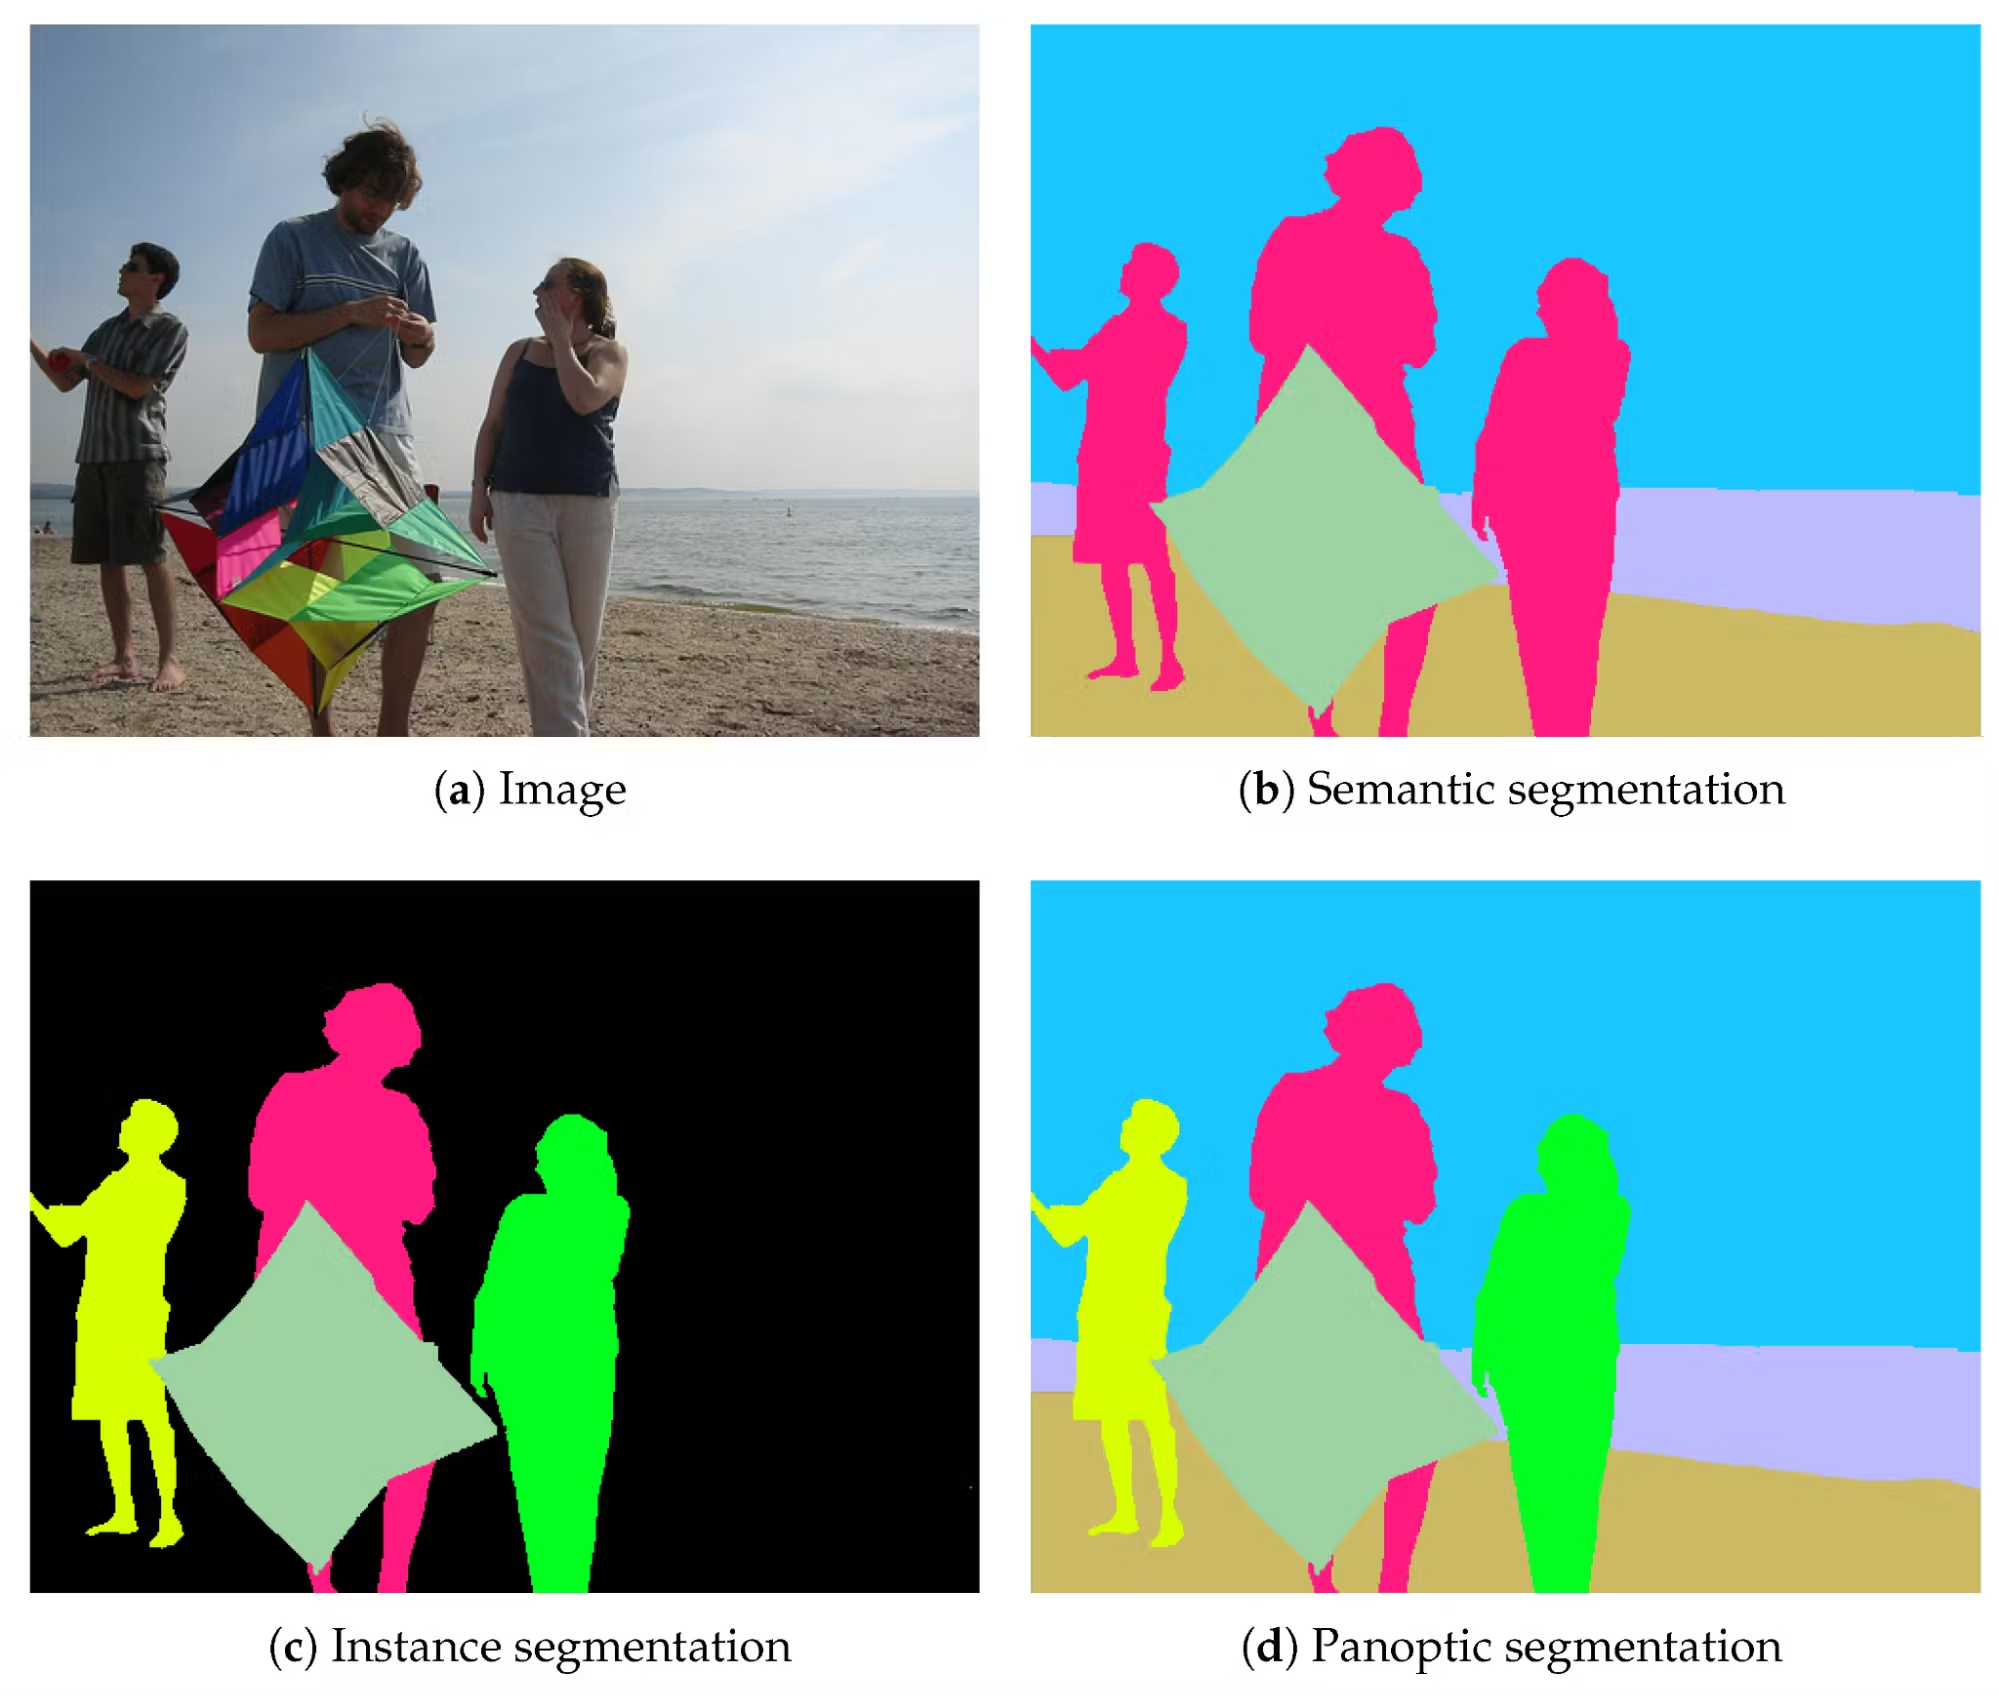
\includegraphics[scale=0.1]{images/segmentation.png}
    \caption{Different types of image segmentation}
    \label{fig:image-segmentation}
\end{figure}

Similarly to object detection, where the Intersection over Union (IoU) metric is widely adopted to evaluate the overlap between predicted and ground-truth bounding boxes, image segmentation relies on pixel-level overlap metrics.
\\
The most commonly used metric is the \textbf{Intersection over Union (IoU)}, also referred to as the \emph{Jaccard Index}. In the context of segmentation, IoU is computed as:

\begin{equation}
IoU = \frac{TP}{TP + FP + FN}
\end{equation}
where:
\begin{itemize}
    \item $TP$ (True Positives) represents the number of correctly predicted pixels belonging to a given class,
    \item $FP$ (False Positives) represents the number of pixels incorrectly assigned to that class,
    \item $FN$ (False Negatives) represents the number of pixels belonging to the class that were not correctly predicted.
\end{itemize}
Another commonly used metric is the \textbf{Dice Coefficient}, also known as the segmentation F1-score, defined as:

\begin{equation}
Dice = \frac{2TP}{2TP + FP + FN}
\end{equation}
The Dice coefficient is particularly popular in medical image segmentation, as it is more sensitive to small objects and class imbalance.

For instance segmentation and panoptic segmentation tasks, additional metrics such as \textbf{Average Precision (AP)} computed over mask IoU thresholds and \textbf{Panoptic Quality (PQ)} are often employed to jointly evaluate detection and segmentation performance.
These evaluation metrics provide a quantitative measure of the agreement between predicted segmentation masks and ground-truth annotations, enabling objective comparison between different models and approaches.
\subsection{Classical segmentation methods}
% !TeX root = ../../tesi.tex

\subsubsection{Clustering}
Clustering is a family of unsupervised methods aimed at grouping data samples according to \textbf{similarity} in a chosen feature space.\cite{mittal_comprehensive_2022} In image analysis, the samples typically correspond to pixels, superpixels, or local feature descriptors, while similarity may be defined in terms of color, intensity, texture, spatial position, or depth.\cite{mittal_comprehensive_2022}

Within computer vision, clustering can be exploited as a classical segmentation strategy.\cite{mittal_comprehensive_2022} The underlying idea is that pixels belonging to the same physical region often share common visual or geometric properties, and can therefore be grouped into homogeneous clusters. Once the clusters have been identified, they can be interpreted as candidate regions of interest or as a first approximation of the object masks.\cite{mittal_comprehensive_2022}

Among the simplest and most widely used approaches is \textbf{k-means clustering}, originally introduced by MacQueen,\cite{macqueen_some_1967} which partitions the input data into $k$ clusters by minimizing the within-cluster variance. When applied to images, k-means can be performed directly on RGB values, grayscale intensities, depth values, or combinations of these features.\cite{macqueen_some_1967,mittal_comprehensive_2022} This makes it particularly useful in scenarios where the target objects can be separated from the background through relatively simple low-level cues.\cite{mittal_comprehensive_2022}

In the present work, clustering is relevant because dough segmentation can benefit from the grouping of pixels or 3D points with similar visual or geometric properties. In the considered setup, color and depth cues can facilitate the separation between the dough and the surrounding scene. In this sense, clustering can be considered a useful classical tool for preprocessing, exploratory segmentation, or the extraction of candidate regions in controlled industrial environments.\cite{mittal_comprehensive_2022}
\begin{figure}[h]
    \centering
    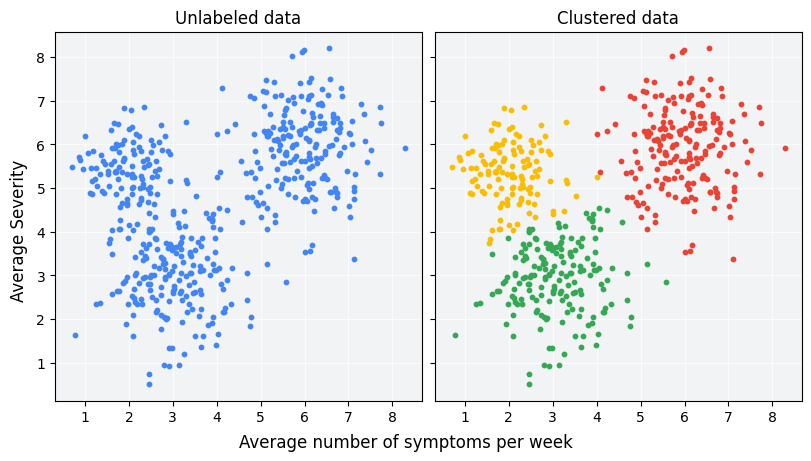
\includegraphics[scale=0.4]{images/clustering.png}
    \caption{Visualization of k-means clustering applied to an image, where pixels are grouped into clusters based on their similarity and distance in the feature-space. Each cluster is represented by a different color, illustrating how the algorithm partitions the image into distinct regions.}
    \label{fig:clustering}
\end{figure}


\subsubsection{Background subtraction}
Background subtraction is another classical strategy for foreground extraction. The main idea is to maintain a model of the background and compare the current observation against it, so as to identify the regions that differ significantly from the static part of the scene.\cite{opencv_background_subtraction_2026}

In vision-based applications, this approach is commonly used with static cameras to generate a foreground mask, that is, a binary image containing the pixels associated with the moving or changing objects in the scene.\cite{opencv_background_subtraction_2026} More generally, the same principle can be extended to cases in which the background is known or can be estimated in advance, and the goal is to isolate the objects of interest by removing the supporting surface or the stationary scene structure.
\begin{figure}[h]
    \centering
    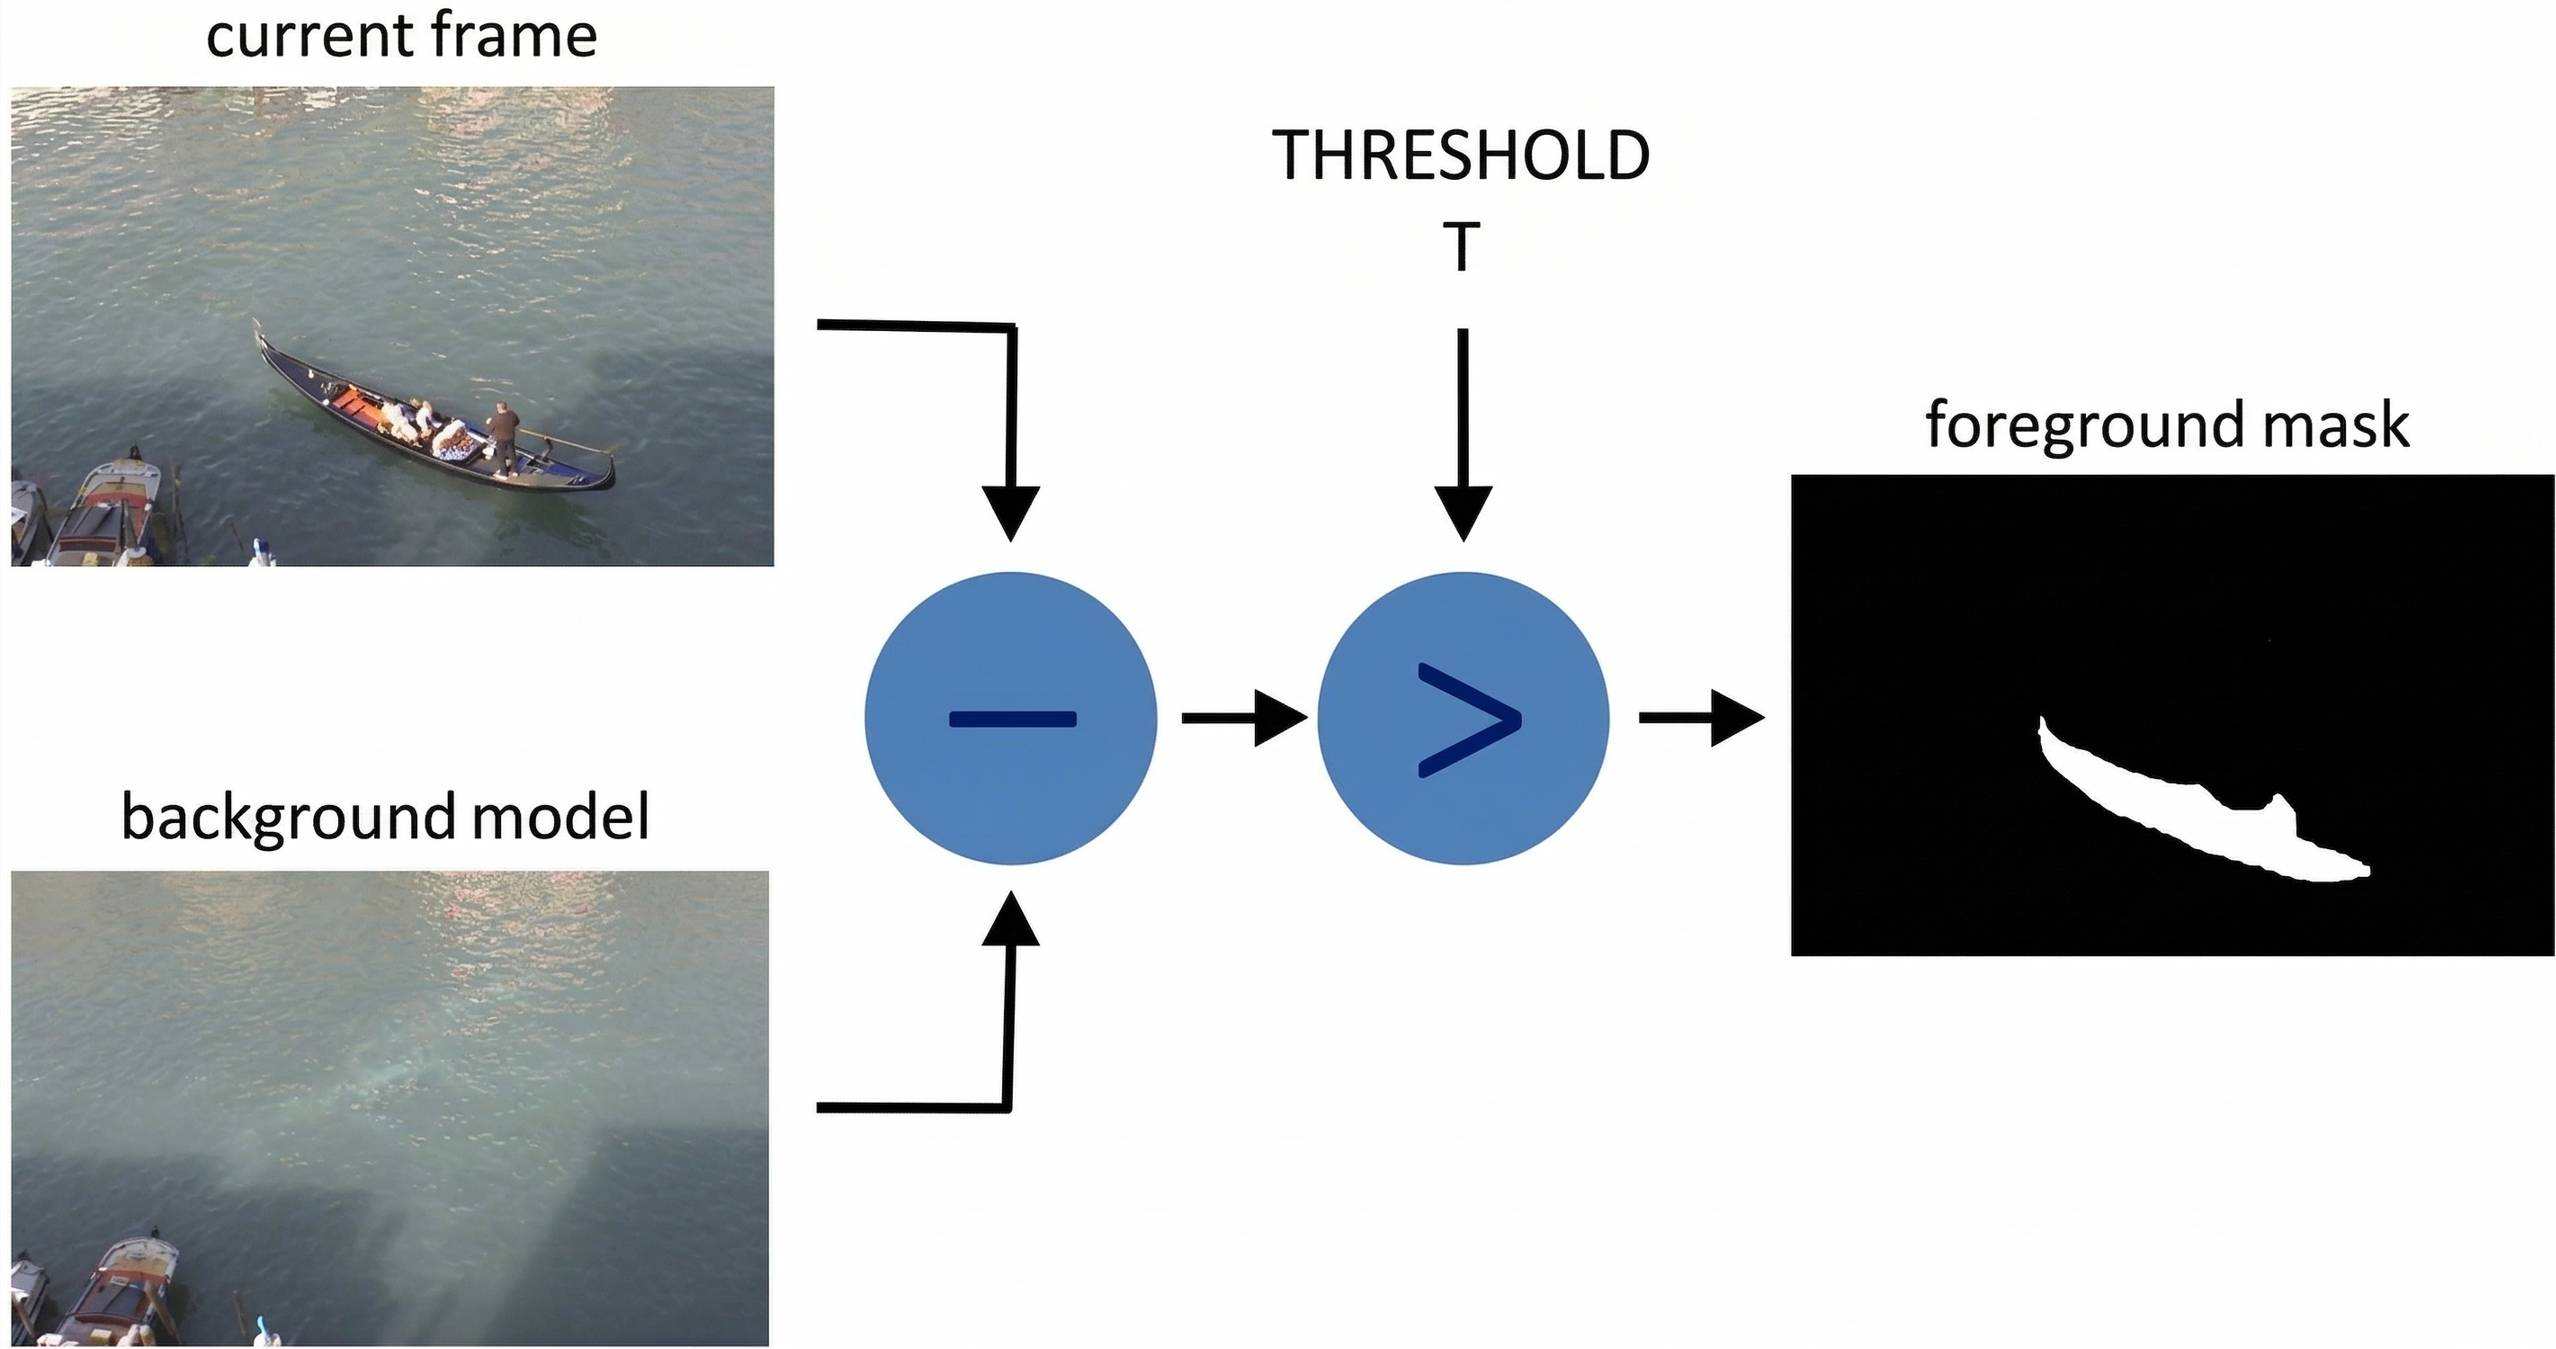
\includegraphics[width=0.6\textwidth]{images/Background_subtraction.png}
    \caption{Background subtraction example scheme.}
    \label{fig:background-subtraction}
\end{figure}

In the present work, this idea is relevant in two complementary ways. First, background subtraction is used in a non segmentation context in the RGB stream as part of the motion-detection module for dataset acquisition. Second, a conceptually similar foreground-background separation is exploited on depth information to isolate the dough from the supporting table before the subsequent geometric analysis.
Since the background (table) is static and can be reliably estimated in depth, this approach provides a computationally efficient way to segment the dough units without relying on complex learning-based models, which may be unnecessary in this controlled setting.

\subsection{Evaluation metrics}
In semantic segmentation, IoU is often computed independently for each class and then averaged across classes, yielding the \textbf{mean Intersection over Union (mIoU)}.\cite{tensorflow_mean_iou_2026,muller_guideline_2022} This metric is particularly informative in multi-class settings because it penalizes both over-segmentation and missed regions.

Other commonly adopted metrics include \textbf{precision} and \textbf{recall}, defined at pixel level as follows:\cite{sklearn_precision_recall_2026}

\begin{equation}
Precision = \frac{TP}{TP + FP}
\end{equation}

\begin{equation}
Recall = \frac{TP}{TP + FN}
\end{equation}

Precision measures how many of the pixels predicted as positive are actually correct, while recall measures how many of the truly positive pixels are successfully retrieved by the model.\cite{sklearn_precision_recall_2026} Their harmonic mean is given by the \textbf{F1-score}, or equivalently the \textbf{Dice coefficient}, which is widely used in segmentation tasks.\cite{muller_guideline_2022}

\begin{equation}
F1 = Dice = \frac{2TP}{2TP + FP + FN}
\end{equation}

In binary segmentation problems or anomaly-detection settings, the \textbf{Area Under the Receiver Operating Characteristic Curve (AUROC)} can also be used. AUROC evaluates the model's ability to discriminate between positive and negative pixels across different decision thresholds.\cite{sklearn_roc_auc_2026} However, in strongly imbalanced segmentation tasks, overlap-based metrics such as IoU or Dice are often considered more informative.\cite{muller_guideline_2022}

For instance segmentation, COCO-style evaluation commonly reports \textbf{Average Precision (AP)} over mask IoU thresholds, while panoptic segmentation is commonly evaluated with \textbf{Panoptic Quality (PQ)}.\cite{detectron2_coco_evaluation_2020,kirillov_panoptic_2019}
These evaluation metrics provide a quantitative measure of the agreement between predicted segmentation masks and ground-truth annotations, enabling objective comparison between different models and approaches.

\section{Neural networks}
% !TeX root = ../../tesi.tex

Neural networks (NNs) are parametric function approximators inspired by the distributed information-processing paradigm of biological nervous systems. At a conceptual level, an NN is composed of interconnected layers of artificial neurons, where each neuron receives a set of inputs, combines them linearly through trainable weights and biases, and then applies a non-linear activation function. By stacking multiple layers, the network implements a nested composition of transformations that can model highly non-linear input--output relationships \cite{goodfellow_deep_2016}. During training, the parameters are adjusted so as to minimize a task-specific loss function, thereby enabling the network to progressively improve its predictions from data \cite{goodfellow_deep_2016}.

\begin{figure}[h]
    \centering
    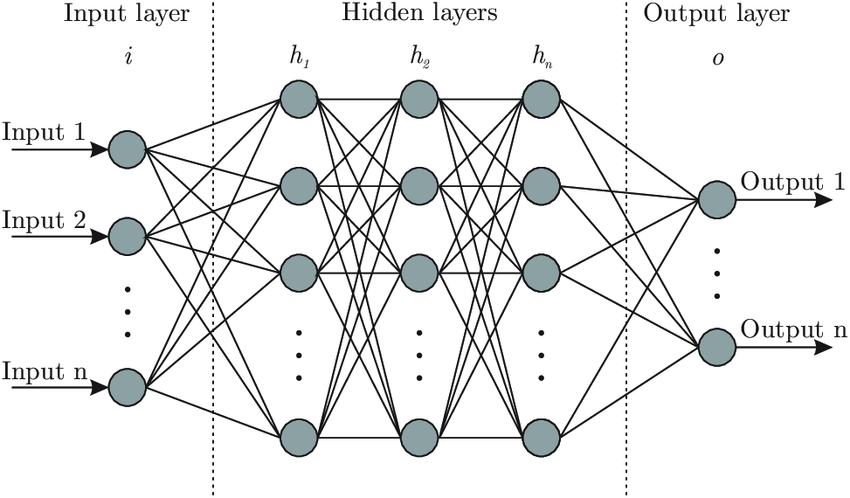
\includegraphics[width=0.5\textwidth]{images/NN.png}
    \caption{Schematic representation of a feedforward neural network with multiple hidden layers. Each layer applies a linear transformation followed by a non-linear activation, enabling progressively richer representations of the input.}
\end{figure}

The optimization of neural networks is typically performed through \textbf{gradient descent} and its stochastic variants. After computing the loss associated with a prediction, gradient descent updates the model parameters in the direction that most reduces the loss, with the size of each update controlled by the learning rate. Backpropagation provides the mechanism that makes this process computationally feasible: by applying the chain rule from the output layer back to the earlier layers, it efficiently computes the gradient of the loss with respect to each parameter in the network \cite{rumelhart_learning_1986,goodfellow_deep_2016}. Together, gradient-based optimization and backpropagation allow neural networks to learn complex functions directly from data.

\begin{figure}[h]
    \centering
    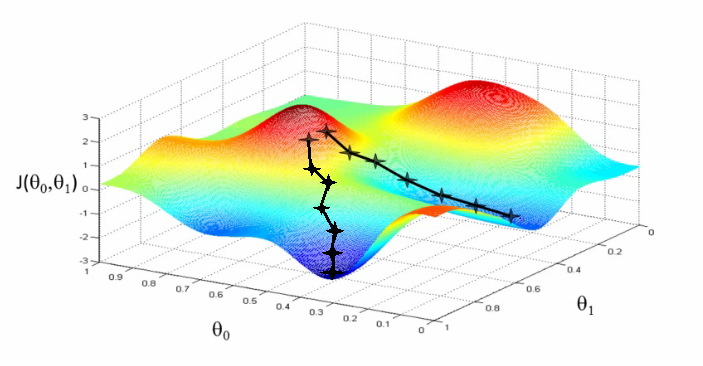
\includegraphics[width=0.5\textwidth]{images/Gradient_descent.png}
    \caption{Illustration of gradient descent over a loss surface. At each iteration, the parameters are updated in the direction of the negative gradient so as to reduce the loss.}
\end{figure}

\subsection{Deep Learning}
While the term neural network refers broadly to a family of trainable models composed of interconnected artificial neurons, \textbf{deep learning} denotes the specific setting in which these models contain multiple representation-learning layers arranged in depth \cite{goodfellow_deep_2016}. The practical importance of depth lies in its ability to learn hierarchical representations: lower layers tend to encode simpler patterns, whereas deeper layers combine them into progressively more abstract and task-relevant features \cite{lecun_deep_2015,goodfellow_deep_2016}. This property distinguishes deep learning from earlier machine learning pipelines, in which feature extraction was often designed manually before classification or regression.

By making end-to-end representation learning possible, deep learning allows the model to infer useful features directly from raw or weakly processed data rather than relying on handcrafted descriptors \cite{goodfellow_deep_2016}. This shift has been one of the main reasons for the remarkable progress observed across computer vision, speech, and natural language processing. At the same time, the high representational capacity of deep models generally \textbf{requires large datasets}, substantial computational resources, and careful optimization procedures in order to achieve strong generalization performance \cite{lecun_deep_2015}. A decisive milestone in this development was the success of deep convolutional networks in large-scale visual recognition, which accelerated both scientific interest and industrial adoption \cite{krizhevsky_imagenet_2012}.
\begin{figure}[h]
    \centering
    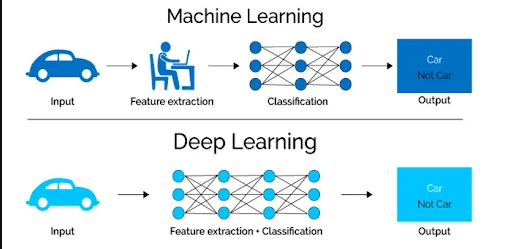
\includegraphics[width=0.5\textwidth]{images/DL.png}
    \caption{Schematic representation of a deep neural network, where feature representations are learned across multiple layers of abstraction and not manually engineered.}
\end{figure}

\subsection{Convolutional Neural Networks}
Among deep architectures for visual data, \textbf{Convolutional Neural Networks (CNNs)} have long represented the dominant paradigm. Their design is based on local receptive fields, \textbf{shared convolutional kernels}, and hierarchical feature extraction as for deep learning nets, which introduce useful inductive biases such as translation equivariance and improved parameter efficiency \cite{lecun_gradient-based_1998,goodfellow_deep_2016}. In a convolutional layer, the same learnable kernel is applied across different spatial positions of the input image, producing feature maps that respond to recurring \textbf{local patterns}. This combination of local connectivity and parameter sharing drastically reduces the number of trainable parameters, making CNNs more efficient to optimize and, in many practical settings, less data-hungry than generic dense architectures for visual tasks \cite{goodfellow_deep_2016,lecun_gradient-based_1998}. 

The use of kernels is particularly well suited to images because relevant visual structures, such as edges, corners, textures, and simple shapes, are inherently local. By learning detectors for these local patterns and reusing them across the whole image, CNNs can extract meaningful features while preserving spatial structure. This property generally improves generalization to unseen images and makes CNNs effective even when computational resources or dataset sizes are more limited than those required by less structured architectures \cite{goodfellow_deep_2016,lecun_gradient-based_1998}. In practice, early layers tend to capture low-level structures, whereas deeper layers encode increasingly abstract semantic patterns. Additional operations such as spatial downsampling or pooling further enlarge the effective receptive field and support the progressive aggregation of information across layers \cite{lecun_gradient-based_1998}. This hierarchical organization explains the effectiveness of CNNs in tasks such as image classification, object detection, and semantic segmentation.

\begin{figure}[h]
    \centering
    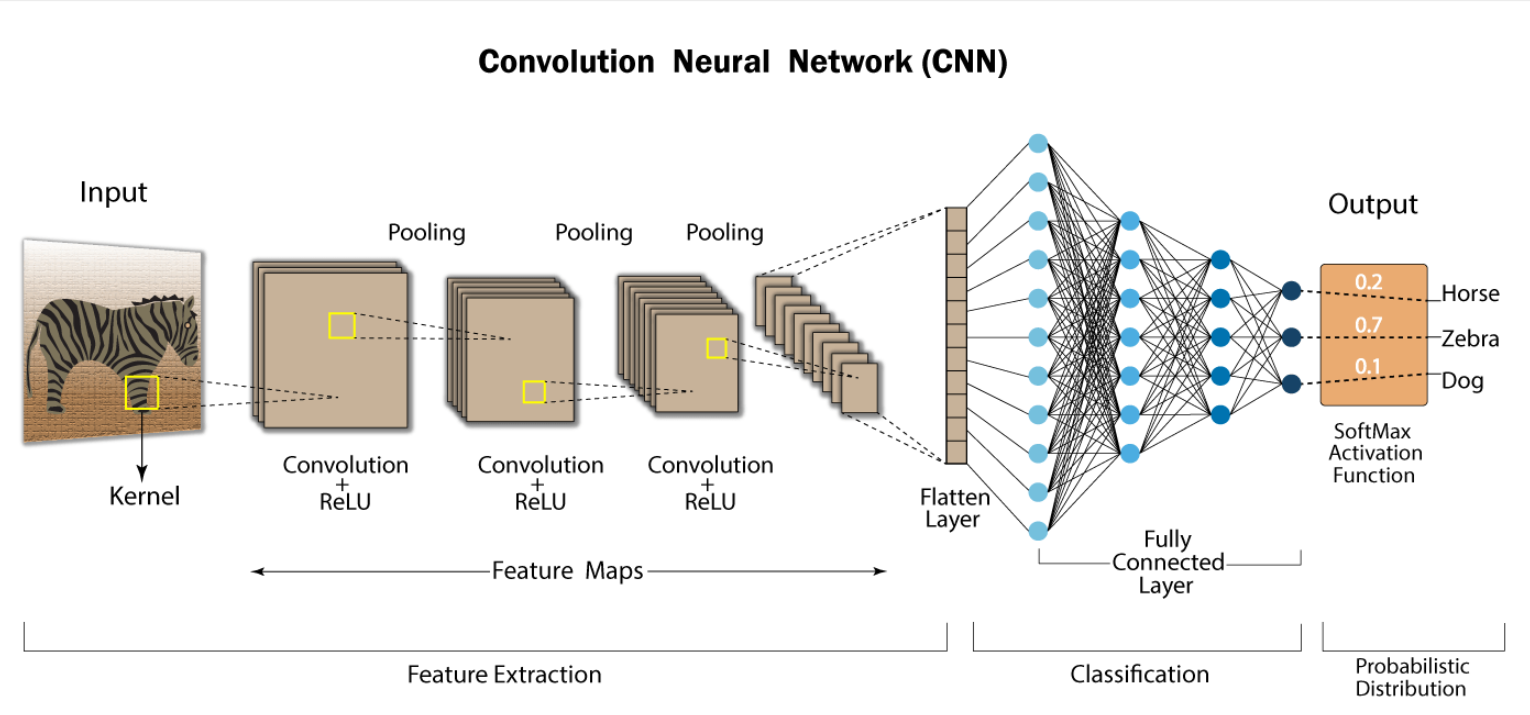
\includegraphics[width=0.52\textwidth]{images/CNN.png}
    \caption{Typical convolutional neural network architecture for visual processing, in which convolutional and downsampling stages progressively extract hierarchical features from the input image.}
\end{figure}

In the context of this thesis, neural networks, deep learning, and CNNs provide the conceptual foundation for the architectures discussed in the following sections. Vision Transformers and RT-DETR will therefore be introduced as successive developments built upon, or reacting to, this baseline \cite{dosovitskiy_image_2021,zhao_detrs_2024}.

\section{Vision Transformers (ViT)}
In recent years, \textbf{Vision Transformers (ViT)} \cite{dosovitskiy_image_2021} have progressively reshaped the landscape of computer vision, offering an alternative to the long-standing dominance of convolutional neural networks (CNNs). Originally inspired by Transformer architectures in natural language processing, ViTs process images as sequences of patches rather than as continuous grids.

More specifically, an input image is divided into fixed-size patches, which are then linearly projected into embedding vectors and treated as tokens. These tokens are processed through a Transformer encoder, where self-attention mechanisms allow the model to capture relationships between distant regions of the image. This ability to model global context is one of the main strengths of ViTs, especially when compared to CNNs, whose receptive field grows only progressively with depth.

This architectural choice brings several advantages. ViTs tend to learn richer semantic representations, making them particularly effective in recognizing complex visual patterns and capturing long-range dependencies. Additionally, their performance scales well with larger datasets and model sizes, often outperforming CNN-based approaches in high-capacity regimes.

However, these benefits come with non-negligible drawbacks. The self-attention operation has a quadratic complexity with respect to the number of tokens, which makes ViTs computationally demanding, especially for high-resolution inputs. This aspect has historically limited their use in real-time or resource-constrained environments.

Despite these limitations, ViTs have become a key component in many modern computer vision pipelines. In particular, they are widely used as backbone networks in object detection and segmentation frameworks, where their ability to extract both global context and fine-grained features proves especially valuable. As also highlighted in the analyzed material \cite{your_pdf_ref}, recent models such as DINO-based architectures demonstrate how ViT backbones can provide strong semantic representations while still being adapted for efficient downstream tasks.
\section{RT-DETR}
% !TeX root = ../../tesi.tex

RT-DETR (Real-Time Detection Transformer) extends the DETR paradigm toward real-time object detection by preserving its end-to-end formulation while explicitly addressing the latency and computational limitations that hindered earlier transformer-based detectors \cite{zhao_detrs_2024}. As in DETR, object detection is formulated as a set prediction problem, so that the model directly outputs a fixed set of detections without relying on heuristic post-processing such as Non-Maximum Suppression (NMS). The main contribution of RT-DETR lies in making this formulation practical for real-time scenarios.
\begin{figure}[h]
    \centering
    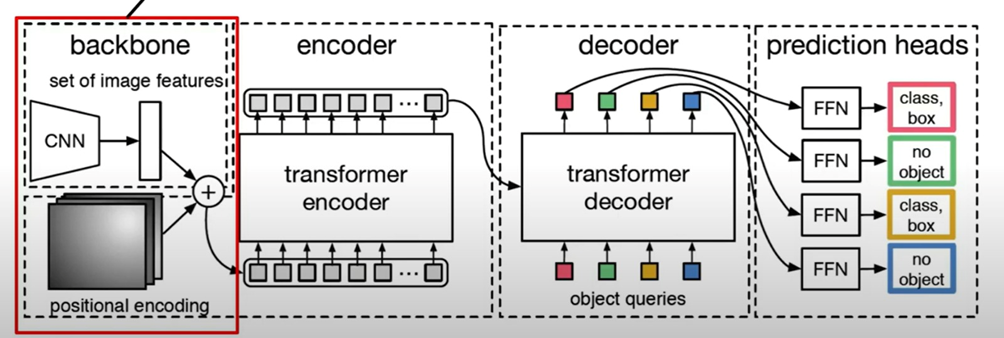
\includegraphics[scale=0.7]{images/DETR.png}
    \caption{Original DETR architecture.}
    \label{fig:DETR_architecture}
\end{figure}

From an architectural perspective, RT-DETR retains the standard backbone--encoder--decoder structure of DETR-style detectors, with prediction heads for object classification and bounding box regression. In this pipeline, the encoder is responsible for processing and fusing the visual features extracted by the backbone, so as to build a more informative representation of the scene before object queries are introduced. The decoder then takes these encoded features together with a set of object queries and iteratively refines them into final detections, progressively improving class predictions and bounding box localization. However, RT-DETR introduces several refinements designed to improve the accuracy--speed trade-off. In particular, the model employs an \textbf{efficient hybrid encoder} to process multi-scale visual features more efficiently by decoupling intra-scale interaction from cross-scale fusion \cite{zhao_detrs_2024}. This design reduces the computational burden of the encoder while still preserving the multi-scale information required for object detection.

\begin{figure}[h]
    \centering
    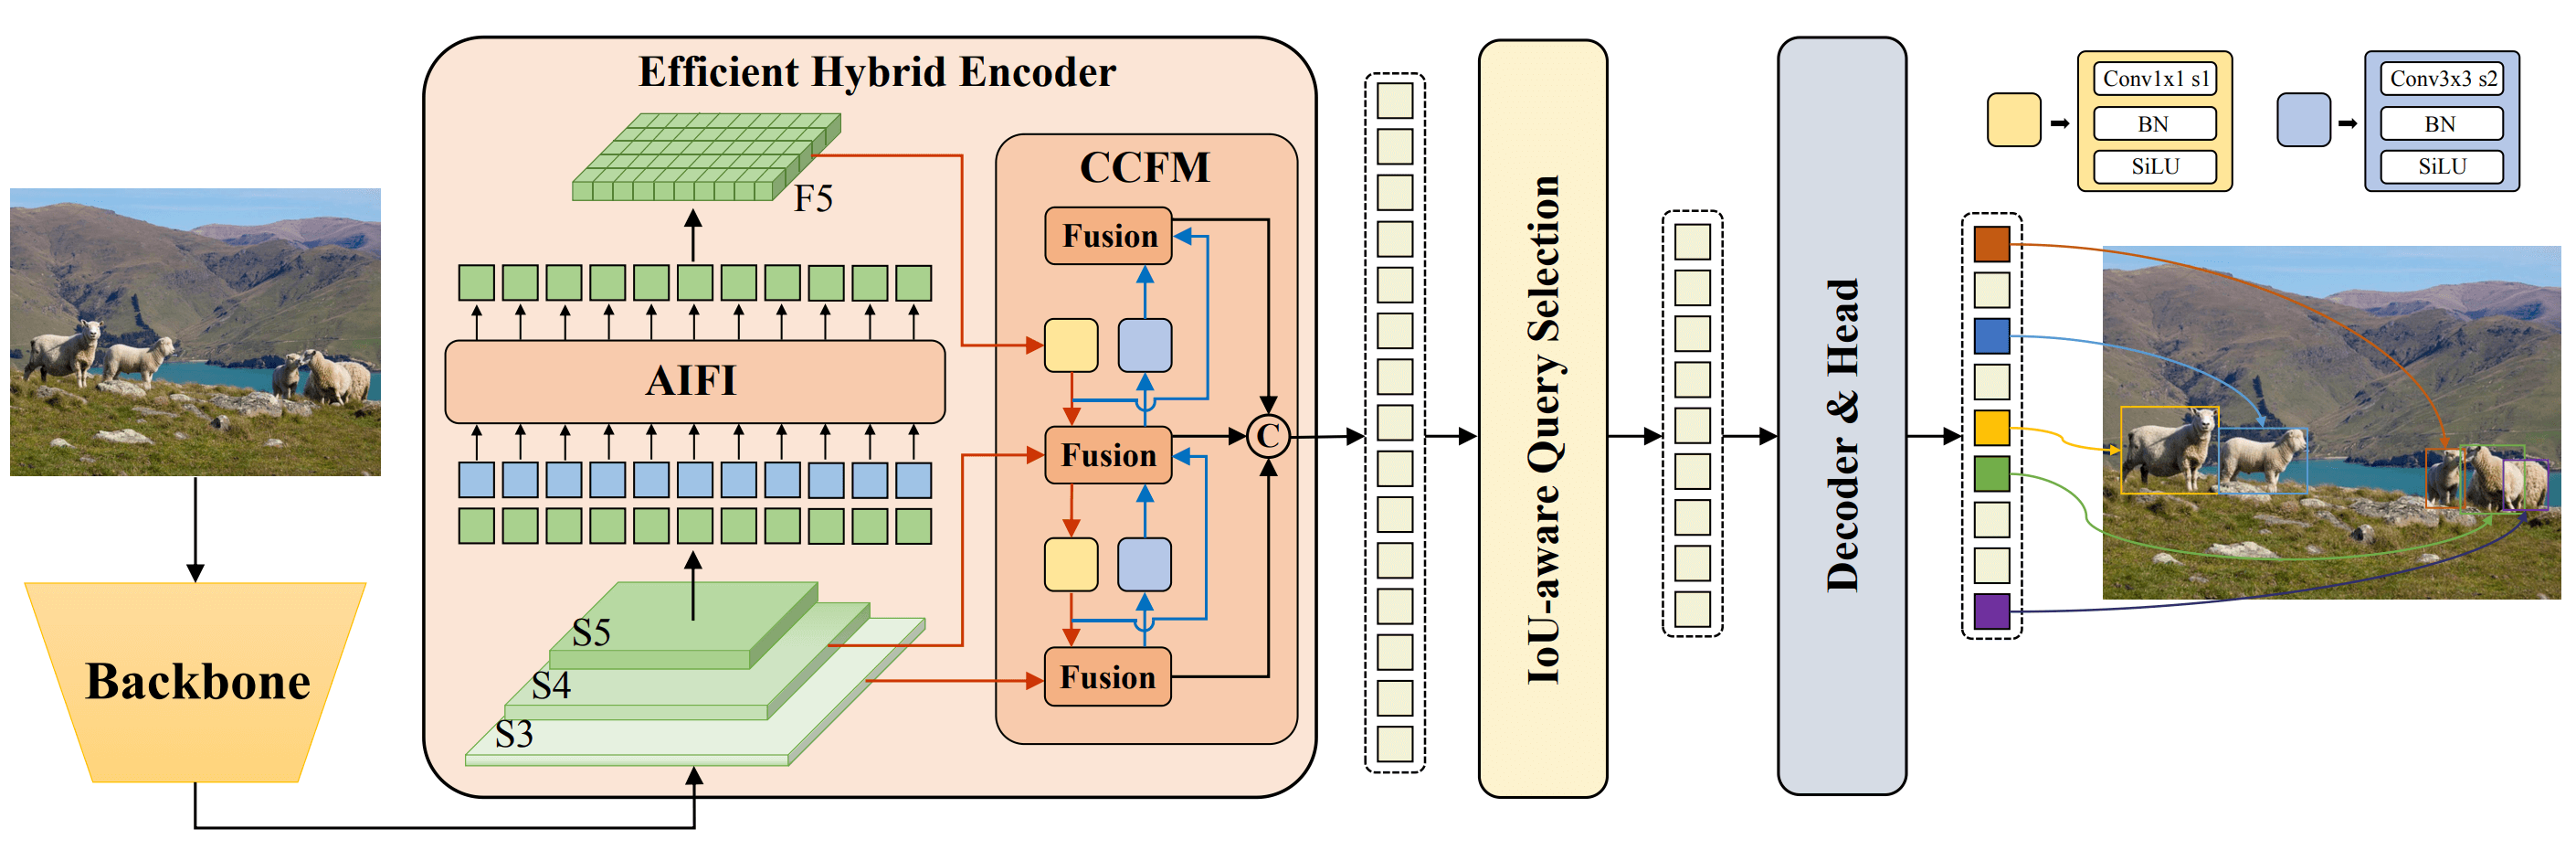
\includegraphics[scale=0.15]{images/RT-DETR.png}
    \caption{RT-DETR architecture.}
    \label{fig:RT-DETR_architecture}
\end{figure}

Another distinctive component is the \textbf{uncertainty-minimal query selection} strategy proposed to initialize the decoder with higher-quality object queries \cite{zhao_detrs_2024}. Rather than forwarding a large set of generic queries, RT-DETR selects encoder features that are expected to be more reliable starting points for detection. Intuitively, the model favors features that are informative both for object classification and for localization, so that the decoder begins its refinement process from more promising candidate regions. This improves efficiency and contributes to stronger detection accuracy.

This query selection mechanism should not be interpreted as a simple hand-crafted thresholding rule, such as selecting all predictions above a fixed IoU value. Instead, it is part of the learned initialization process of the detector and is designed to provide the decoder with a compact set of high-quality queries. After this initialization, the decoder iteratively refines the selected queries into final predictions.

In addition, RT-DETR retains the one-to-one matching paradigm based on the \textbf{Hungarian algorithm}, ensuring that each predicted object is assigned to at most one ground-truth instance during training. This bipartite matching mechanism is central to DETR-style detectors because it removes duplicate assignments and enables an end-to-end detection pipeline without NMS \cite{zhao_detrs_2024}.
\begin{figure}[h]
    \centering
    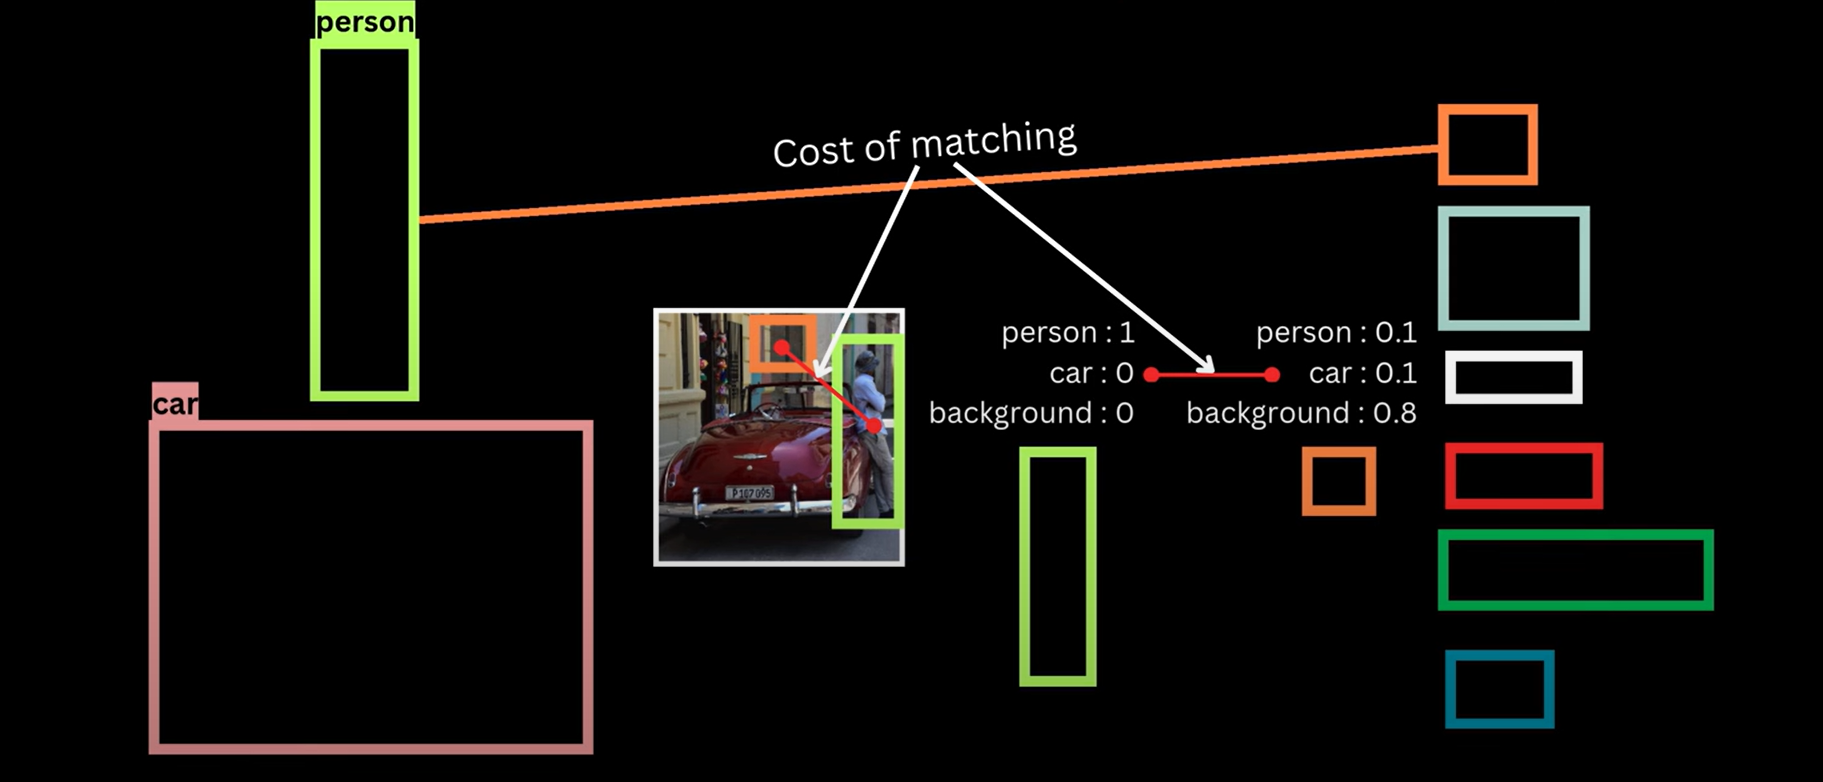
\includegraphics[scale=0.2]{images/Hungarian_match.png}
    \caption{Hungarian matching in RT-DETR.}
    \label{fig:Hungarian_match}
\end{figure}

An additional practical advantage of RT-DETR is its \textbf{flexible speed tuning}: the inference speed can be adjusted by varying the number of decoder layers, allowing the model to adapt to different deployment constraints without retraining \cite{zhao_detrs_2024}. Overall, RT-DETR achieves a strong balance between detection accuracy and computational efficiency, making transformer-based object detection more compatible with real-time and resource-constrained applications. In the context of this thesis, RT-DETR is particularly relevant because it shows how transformer principles can be adapted from generic vision representation learning to an efficient end-to-end detector, while also providing the conceptual basis for subsequent models such as DEIMv2.

\section{Related work}
% !TeX root = ../../tesi.tex

Before selecting the model to be deployed in the proposed inspection pipeline, a comparative literature study was conducted to identify the SOTA architecture that best matched the requirements of this thesis. The analysis focused on three candidate directions: a state-of-the-art real-time detector based on the DETR family (DEIMv2), an attention-centric evolution of the YOLO framework (YOLOv12), and a recent Vision-Transformer-based segmentation model (EoMT). The comparison was guided not only by reported benchmark accuracy, but also by computational cost, parameter efficiency, scalability across hardware regimes, and overall suitability for real-time deployment in the industrial scenarios considered in this work.

\subsection{DEIMv2}
% !TeX root = ../../tesi.tex

DEIMv2 was considered the most direct candidate for this thesis because it explicitly targets the same design space of interest: high-accuracy \emph{real-time} object detection under practical computational constraints \cite{huang_real-time_2026}. Architecturally, DEIMv2 extends the RT-DETR family by combining an end-to-end transformer-based detector with \textbf{stronger backbone features}. 
It offers many variants that span a wide range of model sizes and computational budgets, making it a versatile choice for comparative evaluation. Specifically:
\begin{itemize}
    \item For the mainstream variants (S, M, L, X), it adopts \textbf{DINOv3-pretrained} or distilled Vision Transformer backbones and introduces a \textbf{\emph{Spatial Tuning Adapter} (STA)} to transform the single-scale ViT output into multi-scale features suitable for detection. 

    \item For the ultra-lightweight variants (atto, femto, pico, nano), it instead relies on pruned \textbf{HGNetv2} backbones, thereby covering GPU, edge, and mobile deployment scenarios within the same design family \cite{huang_real-time_2026}.
\end{itemize}
\begin{figure}[h]
    \centering
    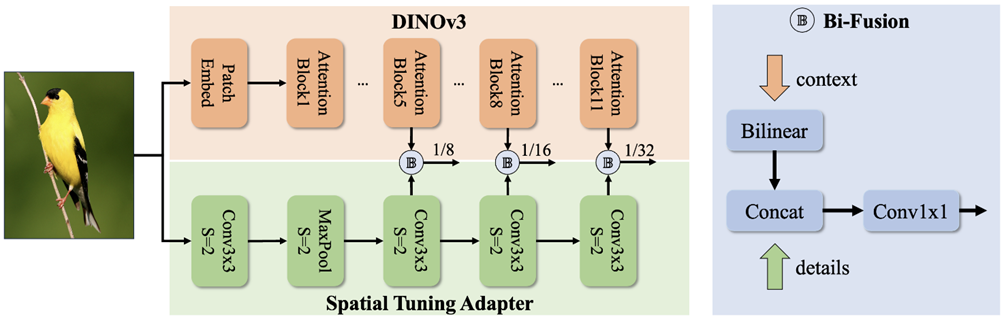
\includegraphics[width=0.8\textwidth]{images/DEIMv2.png}
    \caption{DEIMv2 architecture overview, illustrating the use of DINOv3 backbones and the Spatial Tuning Adapter (STA) to produce multi-scale features for detection \cite{huang_real-time_2026}.}
    \label{fig:DEIMv2_architecture}
\end{figure}

From the perspective of the present application, the main strength of DEIMv2 lies in its ability to combine rich semantic representations with fine-grained local details by integrating DINOv3-based features into an RT-DETR-derived detection framework. This aspect is particularly attractive for the inspection tasks considered in the thesis, since the relevant visual cues may include both global shape information and localized appearance variations. Moreover, DEIMv2 preserves the end-to-end advantages inherited from RT-DETR, including NMS-free prediction, while improving the performance--cost trade-off through stronger features, a simplified decoder, and improved training strategies such as Copy-Blend augmentation \cite{huang_real-time_2026}. The model is also highly scalable: the paper reports strong performance not only for the largest variants, but also for compact versions designed for resource-constrained deployment.
\begin{figure}[h]
    \centering
    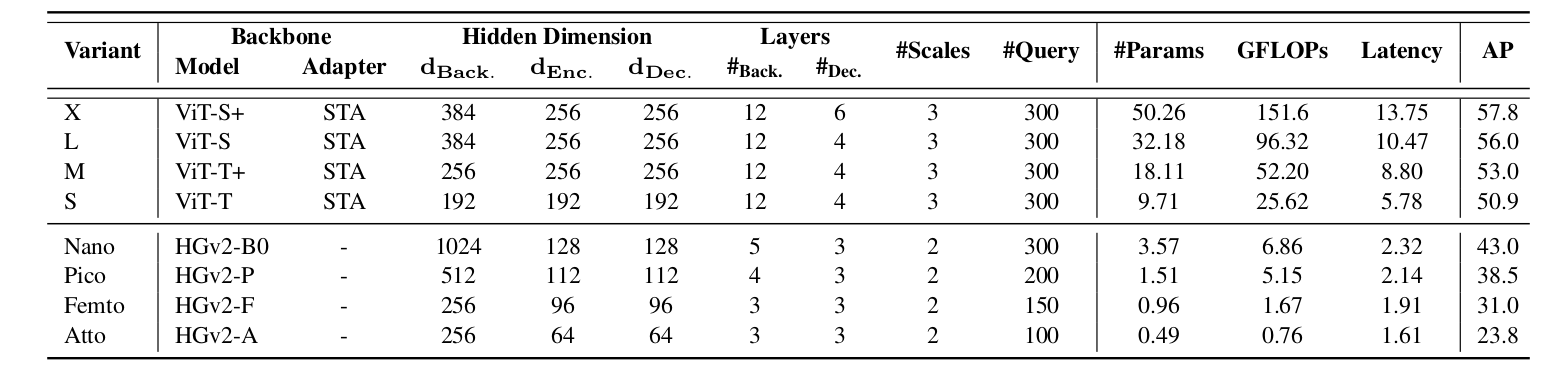
\includegraphics[width=0.9\textwidth]{images/DEIM_results.png}
    \caption{Summary of DEIMv2 results across model scales, highlighting the balance between detection accuracy, latency, and parameter efficiency \cite{huang_real-time_2026}.}
    \label{fig:DEIMv2_results}
\end{figure}

The main limitation of DEIMv2 is that part of its performance advantage depends on the availability of powerful pretrained backbones, especially for the larger variants. In other words, the strongest configurations benefit from large-scale representation learning prior to the downstream detection task. Even so, the model remains particularly compelling within the present comparative study because it combines strong reported accuracy, broad scalability, and clear compatibility with real-time detection requirements \cite{huang_real-time_2026,zhao_detrs_2024}.

\subsection{YOLOv12}
% !TeX root = ../../tesi.tex

YOLOv12 was selected as the main alternative detector because it represents a different and highly competitive design philosophy for real-time object detection \cite{tian_yolov12_2025}. Instead of building on the DETR lineage, YOLOv12 revisits the YOLO framework by introducing an \textbf{\emph{attention-centric}} architecture. Its core idea is to integrate the modeling strength of attention mechanisms into a real-time detector without sacrificing the low-latency behavior that has traditionally made YOLO models attractive in industrial settings. To do so, the paper \cite{tian_yolov12_2025} introduces three key elements: 
\begin{itemize}
    \item \textbf{Area Attention}: A novel attention mechanism that reduces the computational cost of attention by grouping spatial locations into areas, allowing the model to capture long-range dependencies with fewer computations (Figure \ref{fig:YOLOv12_attention}).
    \begin{figure}[h]
        \centering
        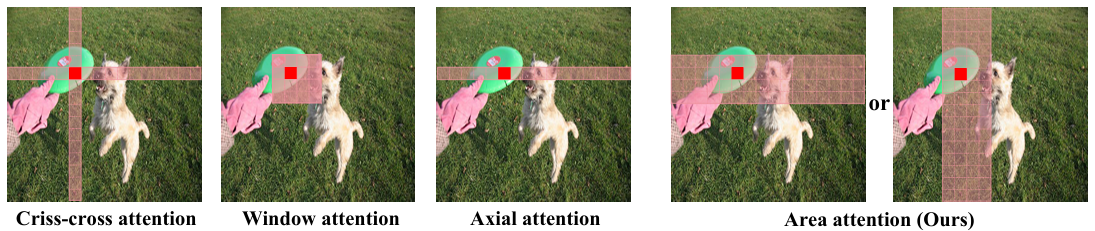
\includegraphics[width=0.9\textwidth]{images/YOLO1.png}
        \caption{Area attention mechanism in YOLOv12 compared to traditional attention mechanisms.}
        \label{fig:YOLOv12_attention}
    \end{figure}
    \item \textbf{R-ELAN}: A modified version of the ELAN architecture that improves optimization stability and convergence in deeper attention-based models, enabling YOLOv12 to scale effectively (Figure \ref{fig:YOLOv12_R-ELAN}).
    \begin{figure}[h]
        \centering
        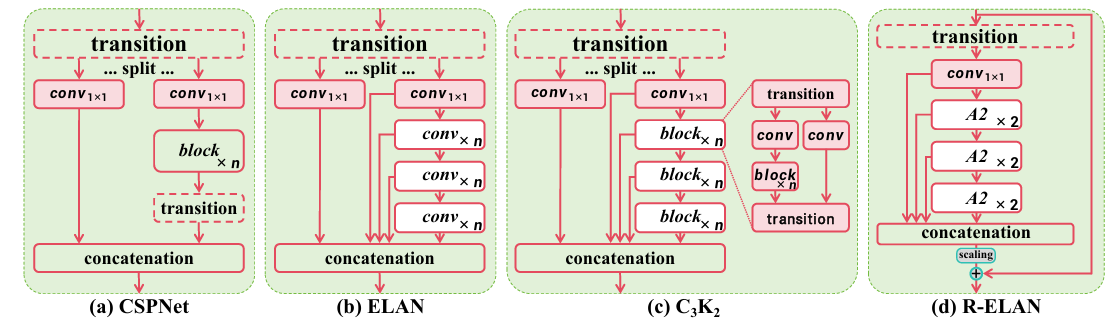
\includegraphics[width=0.9\textwidth]{images/YOLO2.png}
        \caption{YOLOv12 R-ELAN architecture overview, illustrating the skip connection mechanism to improve optimization stability in deeper attention-based models \cite{tian_yolov12_2025}.}
        \label{fig:YOLOv12_R-ELAN}
    \end{figure}
    \item \textbf{FlashAttention}: An efficient implementation of attention that reduces memory-access overhead during inference, further contributing to YOLOv12's low latency.
\end{itemize}

The main appeal of YOLOv12 in the context of this thesis is its excellent latency--accuracy trade-off and its ability to achieve strong results without depending on additional large-scale pretraining strategies. This makes it an attractive candidate whenever extremely low inference time is the primary design criterion. In addition, YOLOv12 is conceptually important because it shows that attention mechanisms can be integrated effectively even within the traditionally convolution-centric YOLO family, thereby challenging the assumption that attention is necessarily too slow for real-time detection \cite{tian_yolov12_2025}.

At the same time, YOLOv12 presents some practical limitations for the specific selection process carried out in this thesis. Its efficiency gains partly depend on hardware support for FlashAttention, which is not equally available across all deployment environments. Furthermore, according to the comparative evidence discussed in the DEIMv2 paper, DEIMv2 later surpassed YOLOv12 in the performance--cost trade-off, achieving higher detection accuracy with fewer parameters and lower computational cost in corresponding regimes \cite{huang_real-time_2026,tian_yolov12_2025}, as showed in Figure \ref{fig:DEIMvsYOLO}. For this reason, YOLOv12 was regarded as a strong benchmark and a valuable reference point, but not as the final choice for deployment.
\begin{figure}[h]
    \centering
    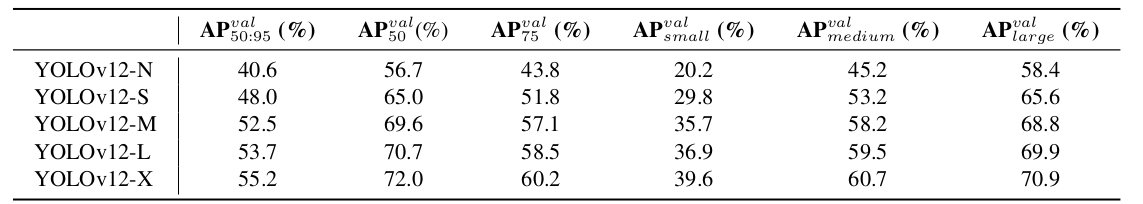
\includegraphics[width=0.9\textwidth]{images/YOLO_results.png}
    \caption{Summary of YOLOv12 results on the COCO benchmark, highlighting its strong balance between detection accuracy and inference efficiency across model scales \cite{tian_yolov12_2025}.}
    \label{fig:YOLOv12_Results}
\end{figure}

\subsection{EoMT}
% !TeX root = ../../tesi.tex

The third candidate direction explored in the literature study was not a detector, but a recent Vision-Transformer-based segmentation model, namely the Encoder-only Mask Transformer (EoMT), introduced in \emph{Your ViT is Secretly an Image Segmentation Model} \cite{kerssies_your_2025}. This work is particularly relevant because it addresses a dense prediction problem that is closely related to object localization, while doing so with a design philosophy aligned with the transformer-based trend discussed in the previous sections. The central idea of EoMT is that, given sufficiently large ViTs and sufficiently strong pretraining, many task-specific segmentation components become less necessary. For this reason, the model removes the convolutional adapter, the pixel decoder, and the separate transformer decoder typically used in ViT-based segmentation pipelines, and replaces them with a simpler encoder-only design augmented by learnable queries and a lightweight mask prediction module \cite{kerssies_your_2025}.

This approach offers several attractive properties. First, it substantially simplifies the segmentation architecture while retaining competitive accuracy. Second, by progressively removing masked attention during training through a \emph{mask annealing} strategy, EoMT enables significantly faster inference than more complex ViT-based segmentation systems. Third, because it stays close to the plain ViT architecture, it can directly benefit from future improvements in large-scale pretraining and transformer optimization \cite{kerssies_your_2025}. From a research standpoint, EoMT was therefore an appealing candidate because it suggested a potentially elegant route toward precise object delineation.

However, the comparative study also highlighted an important mismatch with the main requirements of this thesis. The thesis pipeline ultimately requires robust and efficient \emph{object localization} on embedded or edge-oriented hardware, whereas EoMT is designed for segmentation benchmarks and derives much of its strength from large pretrained ViTs and high-throughput inference settings \cite{kerssies_your_2025}. Although segmentation can provide richer pixel-level information, that additional output is not strictly necessary for the core deployment objective considered here, namely fast localization of dough balls and bread loaves prior to subsequent processing stages. Consequently, EoMT was considered highly interesting from a methodological perspective, but less aligned than DEIMv2 with the operational constraints and output requirements of the thesis.

\subsection{Final considerations}
% !TeX root = ../../tesi.tex

The comparative analysis of the three candidate families revealed a common trend: modern vision systems are increasingly moving beyond purely convolutional designs and are exploiting transformer-based representations in progressively more effective ways. Nevertheless, the final choice could not be based on architectural novelty alone. It had to reflect the concrete needs of the thesis, namely accurate and real-time localization of products in industrial environments, compatibility with edge-oriented deployment, and a favorable balance between predictive performance and computational cost.

Within this framework, DEIMv2 emerged as the most suitable solution. Compared with YOLOv12, it offered a more favorable overall performance--cost trade-off according to the evidence reported in the literature, combining higher detection accuracy with competitive or lower parameter and FLOP budgets in the corresponding model regimes, as illustrated in Figure~\ref{fig:DEIMvsYOLO} \cite{huang_real-time_2026,tian_yolov12_2025}. In addition, its integration of DINOv3-based representations and multi-scale adaptation made it particularly appealing for scenarios in which both local visual details and more global semantic structure may contribute to robust object detection.
Furthermore, DEIMv2's variety of model sizes and its compatibility with real-time detection requirements made it a versatile choice for the different deployment scenarios considered in the thesis, ranging from GPU-based inference to edge-oriented applications \cite{huang_real-time_2026,zhao_detrs_2024}. By contrast, part of YOLOv12's efficiency advantage depends on hardware support for FlashAttention, which is not uniformly available across all deployment environments. In this respect, DEIMv2 appears more flexible and robust as a practical choice for heterogeneous hardware settings.
\begin{figure}[h]
    \centering
    \captionsetup[subfigure]{justification=centering}
    \begin{subfigure}[t]{0.48\textwidth}
        \centering
        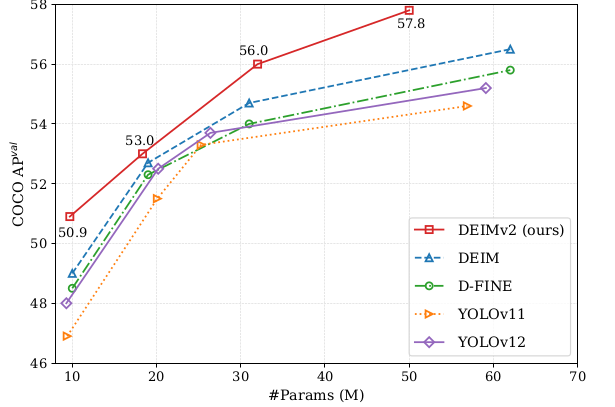
\includegraphics[width=\textwidth]{images/DEIMvsYOLO1.png}
        \caption[c]{Accuracy versus number of parameters for DEIMv2 and YOLOv12 across model scales \cite{huang_real-time_2026,tian_yolov12_2025}.}
        \label{fig:DEIMvsYOLO1}    
    \end{subfigure}\hfill
    \begin{subfigure}[t]{0.48\textwidth}
        \centering
        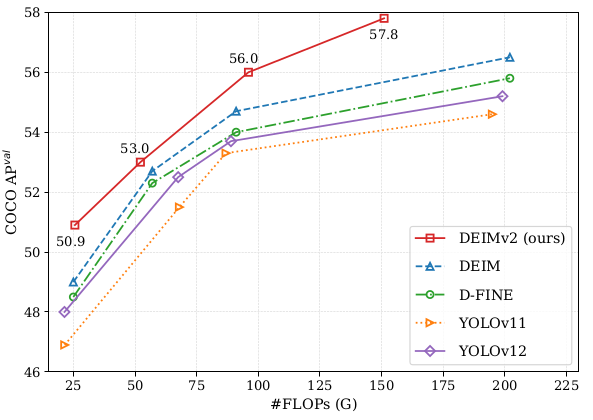
\includegraphics[width=\textwidth]{images/DEIMvsYOLO2.png}
        \caption[c]{Accuracy versus computational cost for DEIMv2 and YOLOv12 across model scales \cite{huang_real-time_2026,tian_yolov12_2025}.}
        \label{fig:DEIMvsYOLO2}
    \end{subfigure}
    \caption{Comparison between DEIMv2 and YOLOv12 in terms of accuracy, parameter count, and computational cost, highlighting the stronger overall efficiency of DEIMv2 across the considered model scales \cite{huang_real-time_2026,tian_yolov12_2025}.}
    \label{fig:DEIMvsYOLO}
\end{figure}

The comparison with EoMT requires a different interpretation, because EoMT addresses image segmentation rather than object detection. For this reason, the decisive argument was not that DEIMv2 is universally superior on a common benchmark, but that it is better aligned with the objective of the thesis. In the proposed pipeline, the essential requirement is to localize each dough ball or loaf quickly and reliably, so that subsequent modules can estimate geometric or appearance-based quantities. For this thesis, object detection is therefore the more appropriate output representation: a full segmentation model would provide richer pixel-level information, but at the cost of denser prediction, greater architectural complexity, and weaker compatibility with low-latency embedded deployment. Moreover, the advantages of EoMT are most evident when large pretrained ViTs and high-performance hardware are available, whereas the thesis prioritizes an efficient real-time detector that can be deployed in practical industrial settings \cite{kerssies_your_2025}.

For these reasons, DEIMv2 was selected as the detection model adopted in this thesis. It combines state-of-the-art real-time detection performance, strong scalability across model sizes, and a transformer-based design that remains compatible with the broader evolution of modern vision architectures. At the same time, the study of YOLOv12 and EoMT remained valuable: YOLOv12 highlighted the growing viability of attention-centric real-time detectors, while EoMT showed that large pretrained ViTs can increasingly absorb task-specific dense prediction components. Together, these works provided the conceptual background against which DEIMv2 was identified as the most appropriate choice for this thesis.

\section{Anomaly Detection}
Anomaly detection is the task of identifying samples that deviate significantly from the expected distribution of normal data. In computer vision, this usually means detecting images or regions whose appearance is inconsistent with the visual patterns observed during training. In industrial inspection, anomaly detection is particularly relevant because defective samples are often rare, heterogeneous, and difficult to collect in a representative way.\cite{li_survey_2025}

Depending on the formulation, visual anomaly detection may operate at different levels of granularity. Some methods produce an \textbf{image-level anomaly score}, indicating whether an image is normal or abnormal as a whole, while others also provide a \textbf{pixel-level anomaly map} that localizes suspicious regions. This distinction is important in industrial settings, where both the decision itself and the interpretability of the detected defect can be relevant.\cite{li_survey_2025}

A common scenario in industrial practice is that abundant normal samples are available, whereas anomalous examples are scarce or completely unavailable. For this reason, many modern anomaly detection methods are designed to learn only the distribution of normal data and to treat deviations from that distribution as potential anomalies.\cite{li_survey_2025} This setting is especially attractive when defects are difficult to enumerate in advance or when collecting defective products would be impractical.

From a methodological perspective, deep-learning-based anomaly detection methods can be grouped into several broad families, including reconstruction-based approaches, feature-embedding methods, teacher--student models, memory-bank methods, and hybrid approaches.\cite{li_survey_2025} Although these methods differ in architecture and supervision signals, they share the same central objective: building a representation of normality that makes abnormal patterns stand out at inference time.

\begin{figure}[h]
    \centering
    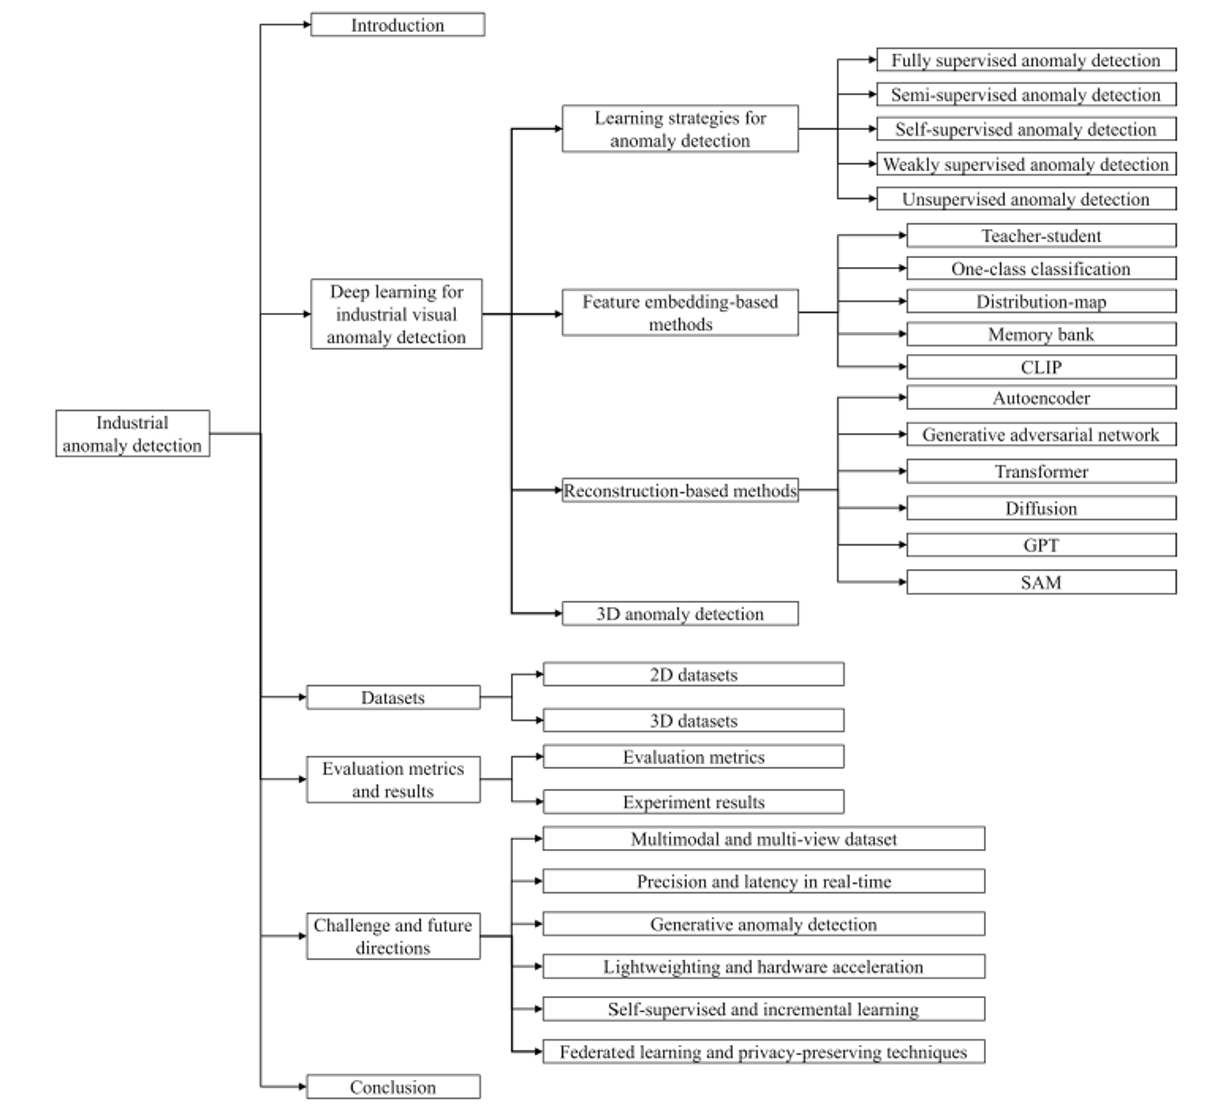
\includegraphics[width=0.9\linewidth]{images/Anomaly.png}
    \caption{Overview of the main methodological families in industrial visual anomaly detection.\cite{li_survey_2025}}
    \label{fig:ivad_taxonomy}
\end{figure}

\subsection{EfficientAD}
Among the anomaly detection methods considered for this thesis, \textbf{EfficientAD} was particularly attractive because it was explicitly designed to achieve a favorable balance between detection accuracy and very low inference latency.\cite{batzner_efficientad_2024} This property is especially important in industrial applications, where anomaly detection must often be integrated into real-time or near-real-time processing pipelines.

At a high level, EfficientAD follows a \textbf{teacher--student paradigm}. A teacher network extracts reference features from normal images, while a student network is trained to reproduce those features on anomaly-free data.\cite{batzner_efficientad_2024} During inference, a large discrepancy between teacher and student representations indicates that the input may contain an anomalous pattern. In addition to this feature-prediction mechanism, EfficientAD incorporates an autoencoder branch to better capture more global or logical anomalies that cannot be explained only through local feature mismatches.\cite{batzner_efficientad_2024}

\begin{figure}[h]
    \centering
    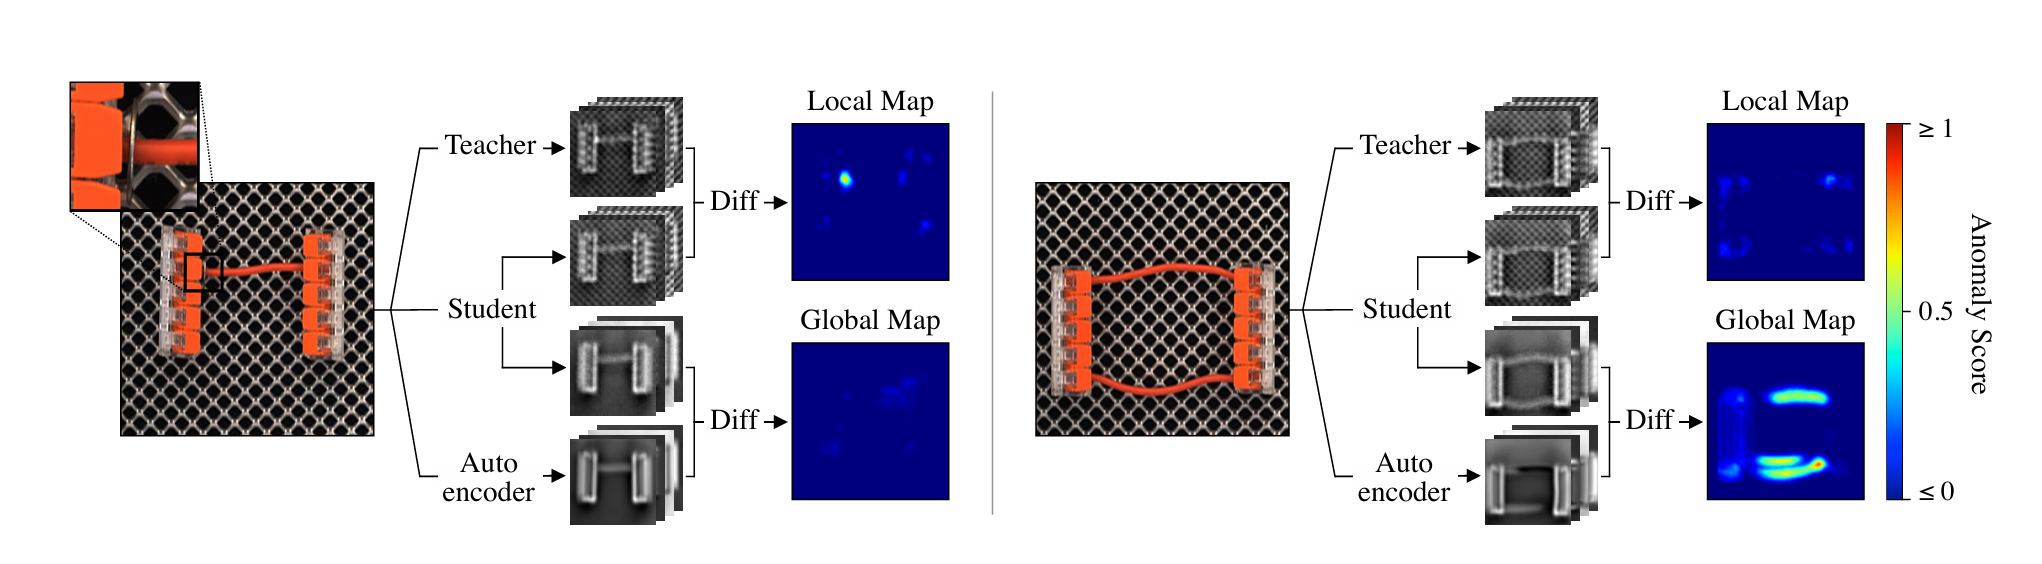
\includegraphics[width=0.95\linewidth]{images/EfficientAD_structure.png}
    \caption{EfficientAD architecture combining teacher--student feature comparison and an autoencoder branch to produce anomaly maps and an image-level anomaly score.\cite{batzner_efficientad_2024}}
    \label{fig:efficientad_architecture}
\end{figure}
\newpage
The main reason for selecting EfficientAD over other anomaly detection methods was therefore practical as well as methodological. First, it is designed for \textbf{high-speed inference}, which makes it suitable for deployment scenarios in which computational resources and response time are both important constraints.\cite{batzner_efficientad_2024} Second, it is available within the \textbf{anomalib} framework, which provides a unified and relatively straightforward implementation environment for state-of-the-art anomaly detection models.\cite{akcay_anomalib_2022} In this sense, EfficientAD offered a combination of efficiency, strong reported performance, and ease of integration that made it particularly convenient for the present work.

Another important aspect is that EfficientAD is well suited to settings in which only normal training samples are available.\cite{batzner_efficientad_2024,li_survey_2025} This makes it particularly relevant for industrial inspection problems in which anomalous data are scarce, poorly characterized, or unavailable during model development. For the purposes of this thesis, this characteristic was especially valuable, because the anomaly detection task had to be framed around learning a reliable representation of normal bread appearance and then measuring deviations from it at inference time.
\begin{figure}[h]
    \centering
    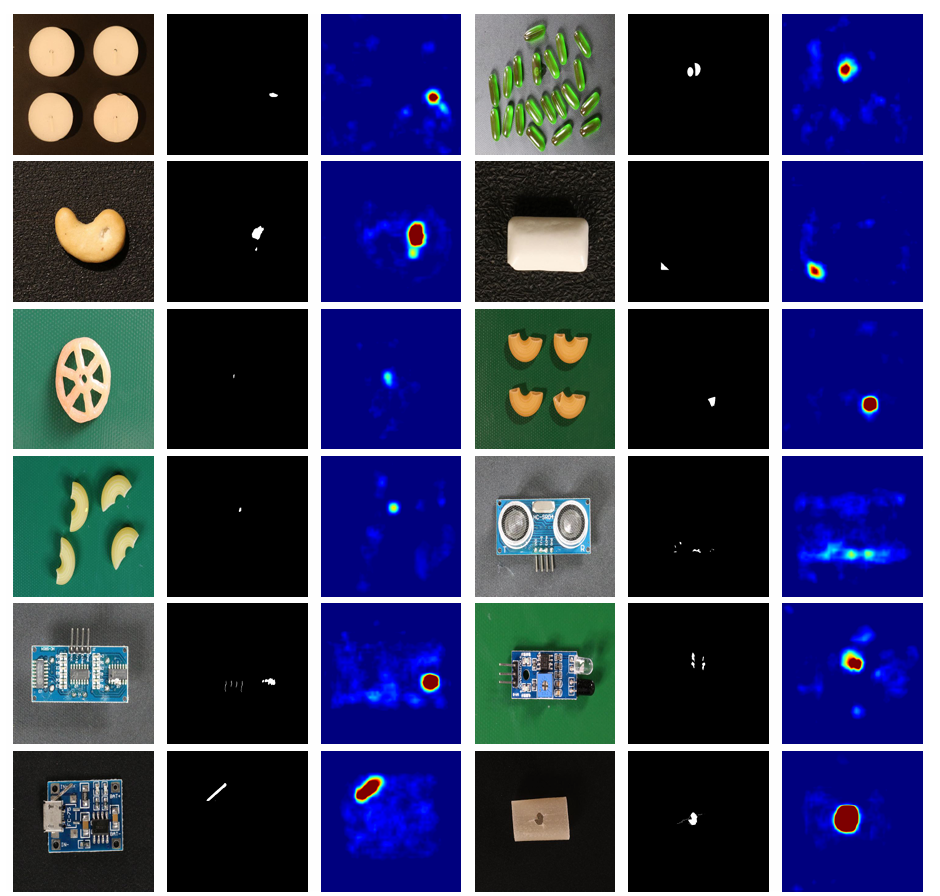
\includegraphics[width=0.6\linewidth]{images/EfficientAD_examples.png}
    \caption{Examples of EfficientAD anomaly maps. The anomalies are highlighted in red, while the normal regions are shown in blue. }
    \label{fig:efficientad_examples}
\end{figure}

\section{Training an AI}
Training a deep learning model consists of iteratively updating its parameters in order to minimize a predefined loss function on the available data.\cite{goodfellow_deep_2016} In supervised and weakly supervised settings, this optimization process is not evaluated solely on the data used for parameter updates, but also on held-out data that provide an estimate of how well the model generalizes to unseen samples.\cite{goodfellow_deep_2016}

For this reason, both the organization of the dataset and the interpretation of training dynamics are central to the development of reliable models. In particular, a clear separation between training, validation, and test data is essential for model selection, while the notions of overfitting and underfitting are fundamental for understanding whether a model is learning meaningful patterns or failing to generalize beyond the training set.\cite{goodfellow_deep_2016}

\subsection{Dataset-split}
A standard practice in machine learning is to divide the available data into at least three subsets: a training set, a validation set, and a test set.\cite{goodfellow_deep_2016} The training set is used to update the model parameters during optimization. The validation set is instead used to monitor generalization during development and to support decisions such as hyperparameter tuning, model selection, and stopping time. Finally, the test set is reserved for the final evaluation of the model and should not influence training decisions.\cite{goodfellow_deep_2016}

The rationale behind this separation is that good performance on the training set alone is not sufficient: the model must also perform well on unseen data. The validation set therefore provides an intermediate estimate of generalization quality while the model is being developed, whereas the test set is used only after the design choices have been fixed.\cite{goodfellow_deep_2016} In practical applications, the exact proportions assigned to these subsets depend on the size and structure of the dataset, and there is no universally optimal split.\cite{sklearn_train_test_split_2026} However, the underlying principle remains the same: parameter learning should be performed on one subset, model selection on another, and final assessment on a third independent subset. This approach helps to prevent overfitting to the training data and ensures that the reported performance metrics reflect the model's ability to generalize to new, unseen examples.\cite{goodfellow_deep_2016}
\begin{figure}[h]
    \centering
    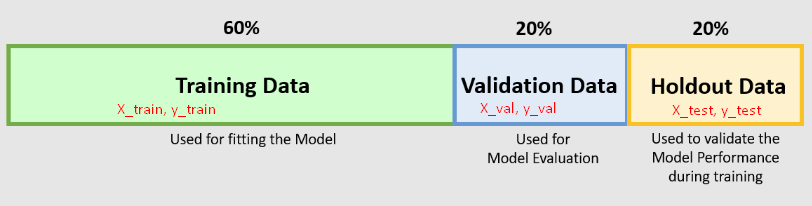
\includegraphics[width=0.85\linewidth]{images/dataset_split.png}
    \caption{Illustration of the standard partition of a dataset into training, validation, and test subsets.}
    \label{fig:dataset_split}
\end{figure}

\subsection{Overfitting-Underfitting}
Two of the central concepts in machine learning are \textbf{underfitting} and \textbf{overfitting}.\cite{goodfellow_deep_2016} Underfitting occurs when a model is unable to achieve sufficiently low error even on the training set. This usually indicates that the model is too simple, insufficiently trained, or poorly configured for the complexity of the task. Overfitting, by contrast, occurs when the model performs very well on the training data but poorly on unseen data, meaning that it has adapted too strongly to idiosyncrasies of the training set rather than learning patterns that generalize.\cite{goodfellow_deep_2016}
\begin{figure}[ht]
    \centering
    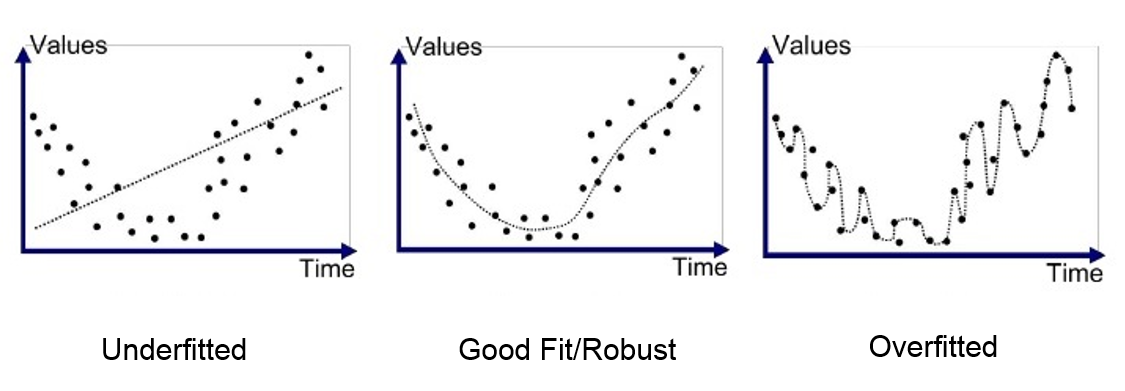
\includegraphics[width=0.75\linewidth]{images/under_over_example.png}
    \caption{Example of underfitting and overfitting in a regression task. The left plot shows an underfitting model that fails to capture the underlying trend, the middle plot shows a well-fitted model that generalizes well, and the right plot shows an overfitting model that captures noise in the training data.}
    \label{fig:example_under_overfitting}
\end{figure}

These two phenomena can often be identified through the evolution of training and validation curves. In an underfitting regime, both training and validation errors remain relatively high. In an overfitting regime, the training error keeps decreasing whereas the validation error stagnates or starts increasing. Monitoring these trends is therefore essential for understanding whether additional training is beneficial or detrimental.\cite{goodfellow_deep_2016,prechelt_early_2012}

One of the most widely used strategies for limiting overfitting is \textbf{early stopping}. During optimization, the training loss may continue to decrease even after the model has already reached its best generalization performance. When the validation error stops improving and begins to worsen, this is a signal that the model is starting to adapt too closely to the training data. Early stopping addresses this issue by interrupting training at the point of best validation performance and retaining the corresponding model parameters.\cite{goodfellow_deep_2016,prechelt_early_2012}
\begin{figure}[ht]
    \centering
    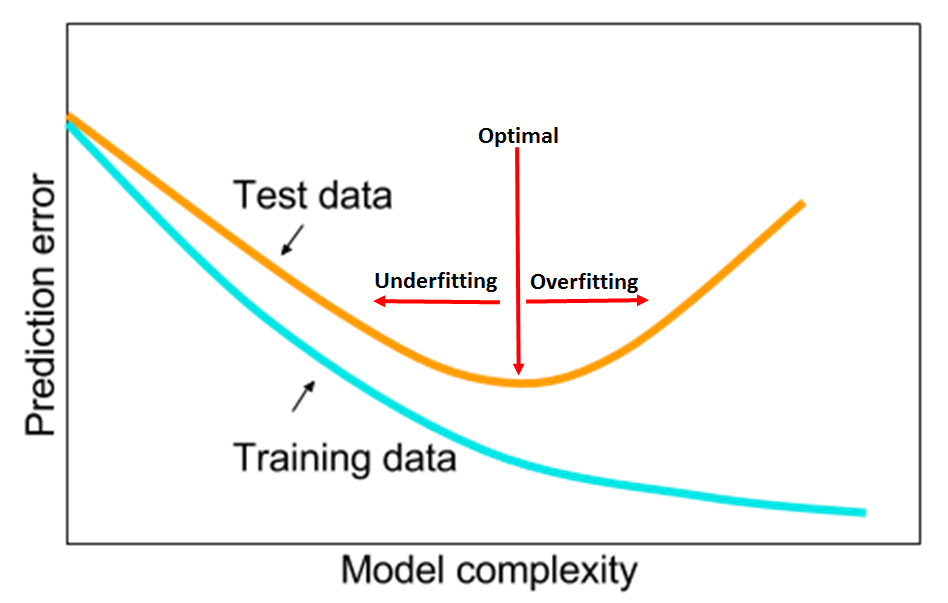
\includegraphics[width=0.6\linewidth]{images/under-overfitting.png}
    \caption{Typical training and validation behaviors in underfitting and overfitting regimes.}
    \label{fig:learning_curves_overfitting}
\end{figure}

Several strategies can be adopted to mitigate these problems. Underfitting may be addressed by increasing model capacity, improving feature quality, extending training, or refining optimization settings. Overfitting can instead be reduced through regularization techniques, data augmentation, early stopping, or, when appropriate, by simplifying the model.\cite{goodfellow_deep_2016} In practice, achieving good generalization requires balancing model capacity and training duration so that the model captures meaningful structure in the data without memorizing the training set.





